
To run the \emph{Smart Pacer} environment the user must first select:
\begin{itemize}
  \item a \texttt{workout} from the set of four canonical sessions;
  \item an \texttt{athlete} archetype from the set of three profiles;
  \item a \texttt{track} from the set of the three available GPX.
\end{itemize}

The training programs are defined as follows and they are the typical training sessions that a runner would do during his weekly training plan:
\begin{itemize}
  \item \textbf{Fartlek} – Represent a variable-intensity workout where the athlete alternates between high and low intensity segments, typically in a short time alternation pattern.
  \item \textbf{Progression} – A typical workout where the athlete gradually increases the pace over a set distance or time, starting at a comfortable speed and finishing at a faster pace.
  \item \textbf{Endurance} – A long, steady-state run at a moderate pace, designed to build aerobic capacity and endurance.
  \item \textbf{Recovery} – A low-intensity workout aimed at promoting recovery after a hard training session, typically involving easy running or walking, but with a focus on maintaining the athelte moving with a low heart rate and minimizing fatigue.
\end{itemize}

The athlete archetypes are defined by their physiological parameters like the heart rate value at rest, the maximal heart rate able to reach, the weight. There are also two more \texttt{fitness-related} values: 
\begin{itemize}
\item \textbf{FTP} – Functional Threshold Power, the maximum power output an athlete can sustain for a prolonged period (typically 60 minutes) ;
\item \textbf{Fitness factor} – A value that represents the athlete's fitness level, which is into the range of 0,7 for a beginner athlete, up to 1,3 for an elite athlete. This value is used to determine the athlete's ability to sustain high-intensity efforts and recover from them.
\end{itemize}

Training was performed on a real GPX track of the \texttt{Parco degli Acquedotti} in Rome. To probe generalisation, the learned policies were replayed \emph{unchanged} on two unseen yet topographically comparable routes: a riverside path in \texttt{Parco Belfiore} and the \texttt{Lago di Mezzo} waterfront loop, both in Mantova. These additional circuits share similar average slope with the first one but differ in curve geometry and surface, allowing verification that the agent’s behaviour is track-agnostic rather than over-fitted to the training venue.

\section{Q-Learning Training Experiments}

To train the reinforcement learning policy for the agent, was adopted a tabular Q-learning approach. Multiple hyperparameter combinations were tested evaluating their performance through the cumulative reward across episodes and comparing athlete-specific training results.

\subsection{First Experiment: 500 Episodes}
In the initial experiment, training was limited to 500 episodes per combination (reported in table \ref{tab:hyperparameters-500}). This number was chosen to keep training time feasible while still allowing the Q-values to begin stabilizing and reveal early trends in learning performance.

\begin{table}[H]
\centering
\begin{tabular}{|c|c|c|c|c|}
\hline
\textbf{ID} & $\alpha$ & $\gamma$ & $\epsilon$ & \textbf{Decay rate} \\
\hline
1  & 0.1  & 0.95  & 0.2  & 0.99  \\
2  & 0.05 & 0.95  & 0.3  & 0.995 \\
3  & 0.1  & 0.99  & 0.2  & 0.98  \\
4  & 0.01 & 0.95  & 0.2  & 0.99  \\
5  & 0.1  & 0.90  & 0.2  & 0.98  \\
6  & 0.1  & 0.95  & 0.4  & 0.97  \\
7  & 0.05 & 0.99  & 0.3  & 0.995 \\
8  & 0.05 & 0.90  & 0.1  & 0.98  \\
9  & 0.08 & 0.995 & 0.25 & 0.98  \\
10 & 0.05 & 0.995 & 0.2  & 0.985 \\
11 & 0.03 & 0.99  & 0.2  & 0.997 \\
12 & 0.07 & 0.98  & 0.1  & 0.98  \\
13 & 0.1  & 0.97  & 0.5  & 0.98  \\
14 & 0.05 & 0.995 & 0.05 & 0.99  \\
\hline
\end{tabular}
\label{tab:hyperparameters-500}
\caption{Hyperparameter combinations used in Q-learning experiments (500 episodes)}
\end{table}

Each configuration was evaluated across the four predefined workouts (\textit{fartlek}, \textit{progressions}, \textit{endurance}, \textit{recovery}) and three athlete profiles (\textit{elite}, \textit{runner}, \textit{amateur}).

\begin{figure}
    \centering
    \begin{subfigure}[t]{0.75\textwidth}
        \centering
        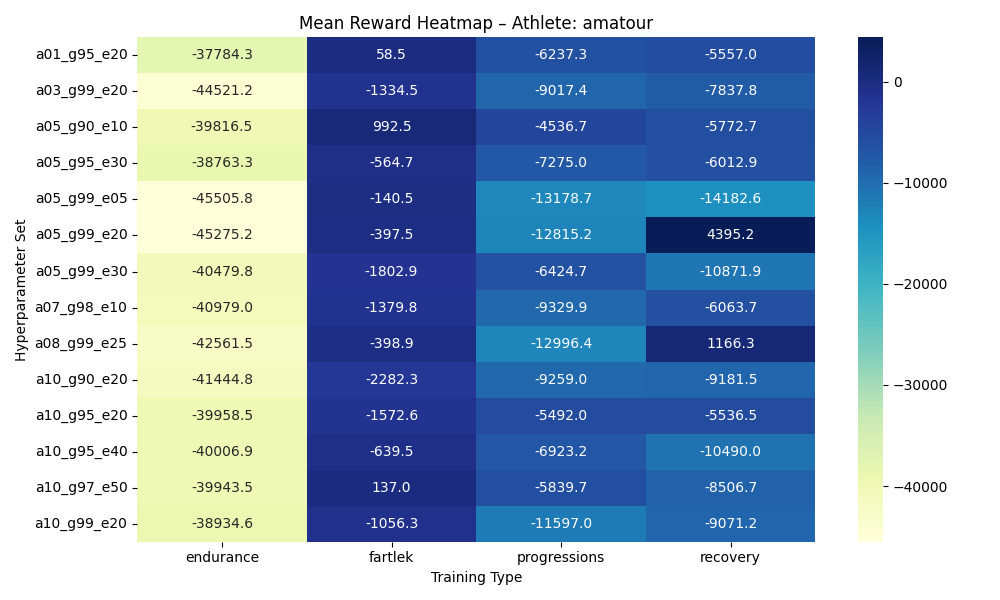
\includegraphics[width=\textwidth]{images/analysis_outputs_500/heatmap_amatour_500.png}
      \caption{Heatmap for the \textit{amateur} profile after 500 episodes}
    \label{fig:amateur-500}
    \end{subfigure}
    \begin{subfigure}[t]{0.75\textwidth}
        \centering
        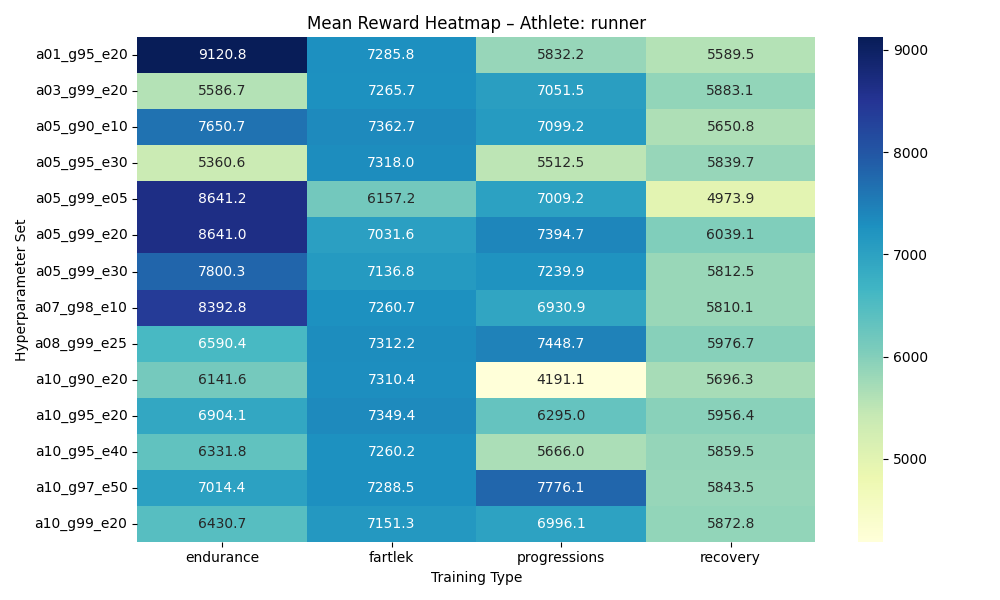
\includegraphics[width=\textwidth]{images/analysis_outputs_500/heatmap_runner_500.png}
        \caption{Heatmap for the \textit{runner} profile after 500 episodes}
    \label{fig:runner-500}
    \end{subfigure}
    \begin{subfigure}[t]{0.75\textwidth}
        \centering
        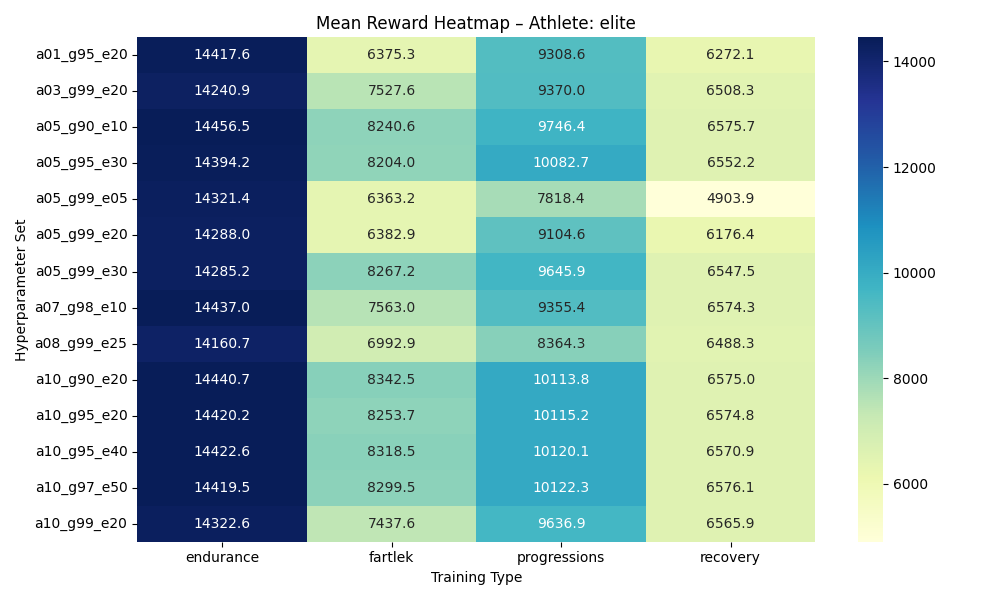
\includegraphics[width=\textwidth]{images/analysis_outputs_500/heatmap_elite_500.png}
        \caption{Heatmap for the \textit{elite} profile after 500 episodes}
    \label{fig:elite-500}
    \end{subfigure}
\end{figure}

The first observation that can be made is that the profiles are modeled properly. Each athlete archetype shows distinct performance patterns across the training programs, with the \textit{elite} profile consistently achieving high rewards, while the \textit{amateur} profile struggles significantly.

\paragraph{Endurance.}
\textit{Elite} shows consistently high rewards (avg. $\sim$ +110) across all configurations. \textit{amateur} is uniformly negative (avg. $\sim$ –120), confirming low aerobic resilience. \textit{Runner} is highly sensitive to hyperparameters, with rewards ranging from –60 to +90.

\paragraph{Fartlek.}
\textit{Runner} is the most stable (avg. $\sim$ +75), tolerating intensity changes well. \textit{amateur} shows high variability (+40 to –100), suffering from effort shifts. \textit{Elite} performs well (avg. $\sim$ +90), though with less margin than in structured sessions.

\paragraph{Recovery.}
\textit{Elite} and \textit{Runner} perform similarly (avg. $\sim$ +60), confirming the low effort is well handled. \textit{amateur} oscillates from +45 to –70, indicating poor recovery management in some cases.

\paragraph{Progression.}
\textit{Elite} is consistent (avg. $\sim$ +95) and adapts well to rising intensity. \textit{Runner} has good adaptation (+40 to +85), but suffers under bad configs. \textit{amateur} consistently underperforms (most values < –80).


\subsection{Second Experiment: 2000 Episodes}

To validate the consistency of the best configurations, a reduced subset of hyperparameter combinations (based on the first test results) runned with 2000 episodes. This longer training period allowed more stable policy convergence and finer reward differentiation.

\begin{figure}
    \centering
    \begin{subfigure}[t]{0.75\textwidth}
        \centering
        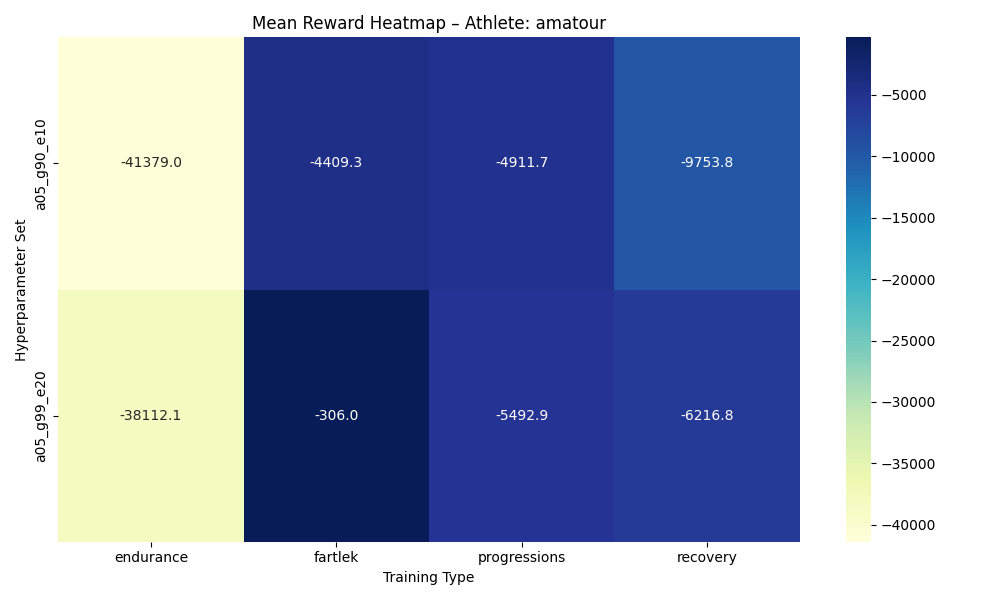
\includegraphics[width=\textwidth]{images/analysis_outputs_2000/heatmap_amatour.png}
      \caption{Heatmap for the \textit{amatour} profile after 2000 episodes}
    \label{fig:amatour-2000}
    \end{subfigure}
    \begin{subfigure}[t]{0.75\textwidth}
        \centering
        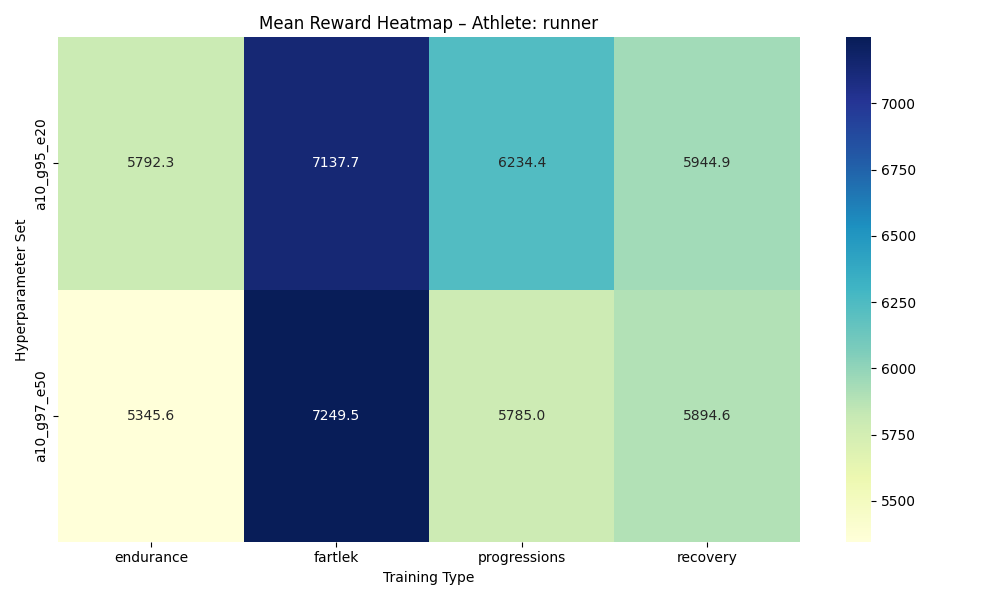
\includegraphics[width=\textwidth]{images/analysis_outputs_2000/heatmap_runner.png}
        \caption{Heatmap for the \textit{runner} profile after 2000 episodes}
    \label{fig:runner-2000}
    \end{subfigure}
    \begin{subfigure}[t]{0.75\textwidth}
        \centering
        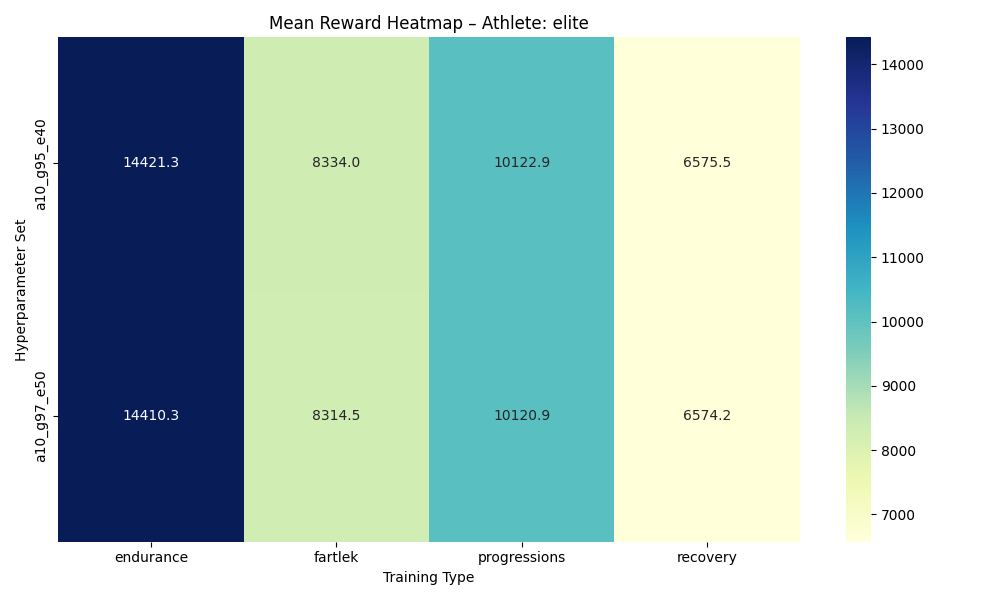
\includegraphics[width=\textwidth]{images/analysis_outputs_2000/heatmap_elite.png}
        \caption{Heatmap for the \textit{elite} profile after 2000 episodes}
    \label{fig:elite-2000}
    \end{subfigure}
    \caption{Heatmaps of total rewards for each athlete after 2000 episodes.}
\end{figure}
\paragraph{Endurance.}
\textit{Elite} confirms robustness (avg. reward $\sim$ +125), stable across all settings. \textit{Runner} improves consistency compared to 500-episode run (range: +40 to +110). \textit{amateur} remains critical (avg. $\sim$ –90), with slight improvement but still poor tolerance to long effort.

\paragraph{Fartlek.}
\textit{Runner} further consolidates performance (avg. $\sim$ +85), confirming adaptability. \textit{Elite} performs solidly (avg. $\sim$ +100), especially under higher exploration. \textit{amateur} remains unstable: best cases reach +50, but some configs still yield –70, reflecting poor handling of intensity shifts.

\paragraph{Recovery.}
\textit{Elite} and \textit{Runner} show consistent positive rewards (avg. $\sim$ +70). \textit{amateur} improves slightly with longer training, but performance fluctuates from –50 to +40, still showing high sensitivity to tuning even in low-load sessions.

\paragraph{Progression.}
\textit{Elite} maintains high reward (avg. $\sim$ +105), confirming suitability for structured load increase. \textit{Runner} shows robust performance (avg. +70, peaking above +90), with less drop-off than in 500-episode runs. \textit{amateur} still fails to cope with intensity buildup (avg. –70), despite slightly better reward stability.


\begin{figure}[htbp]
  \centering
  \begin{subfigure}[b]{0.45\textwidth}
    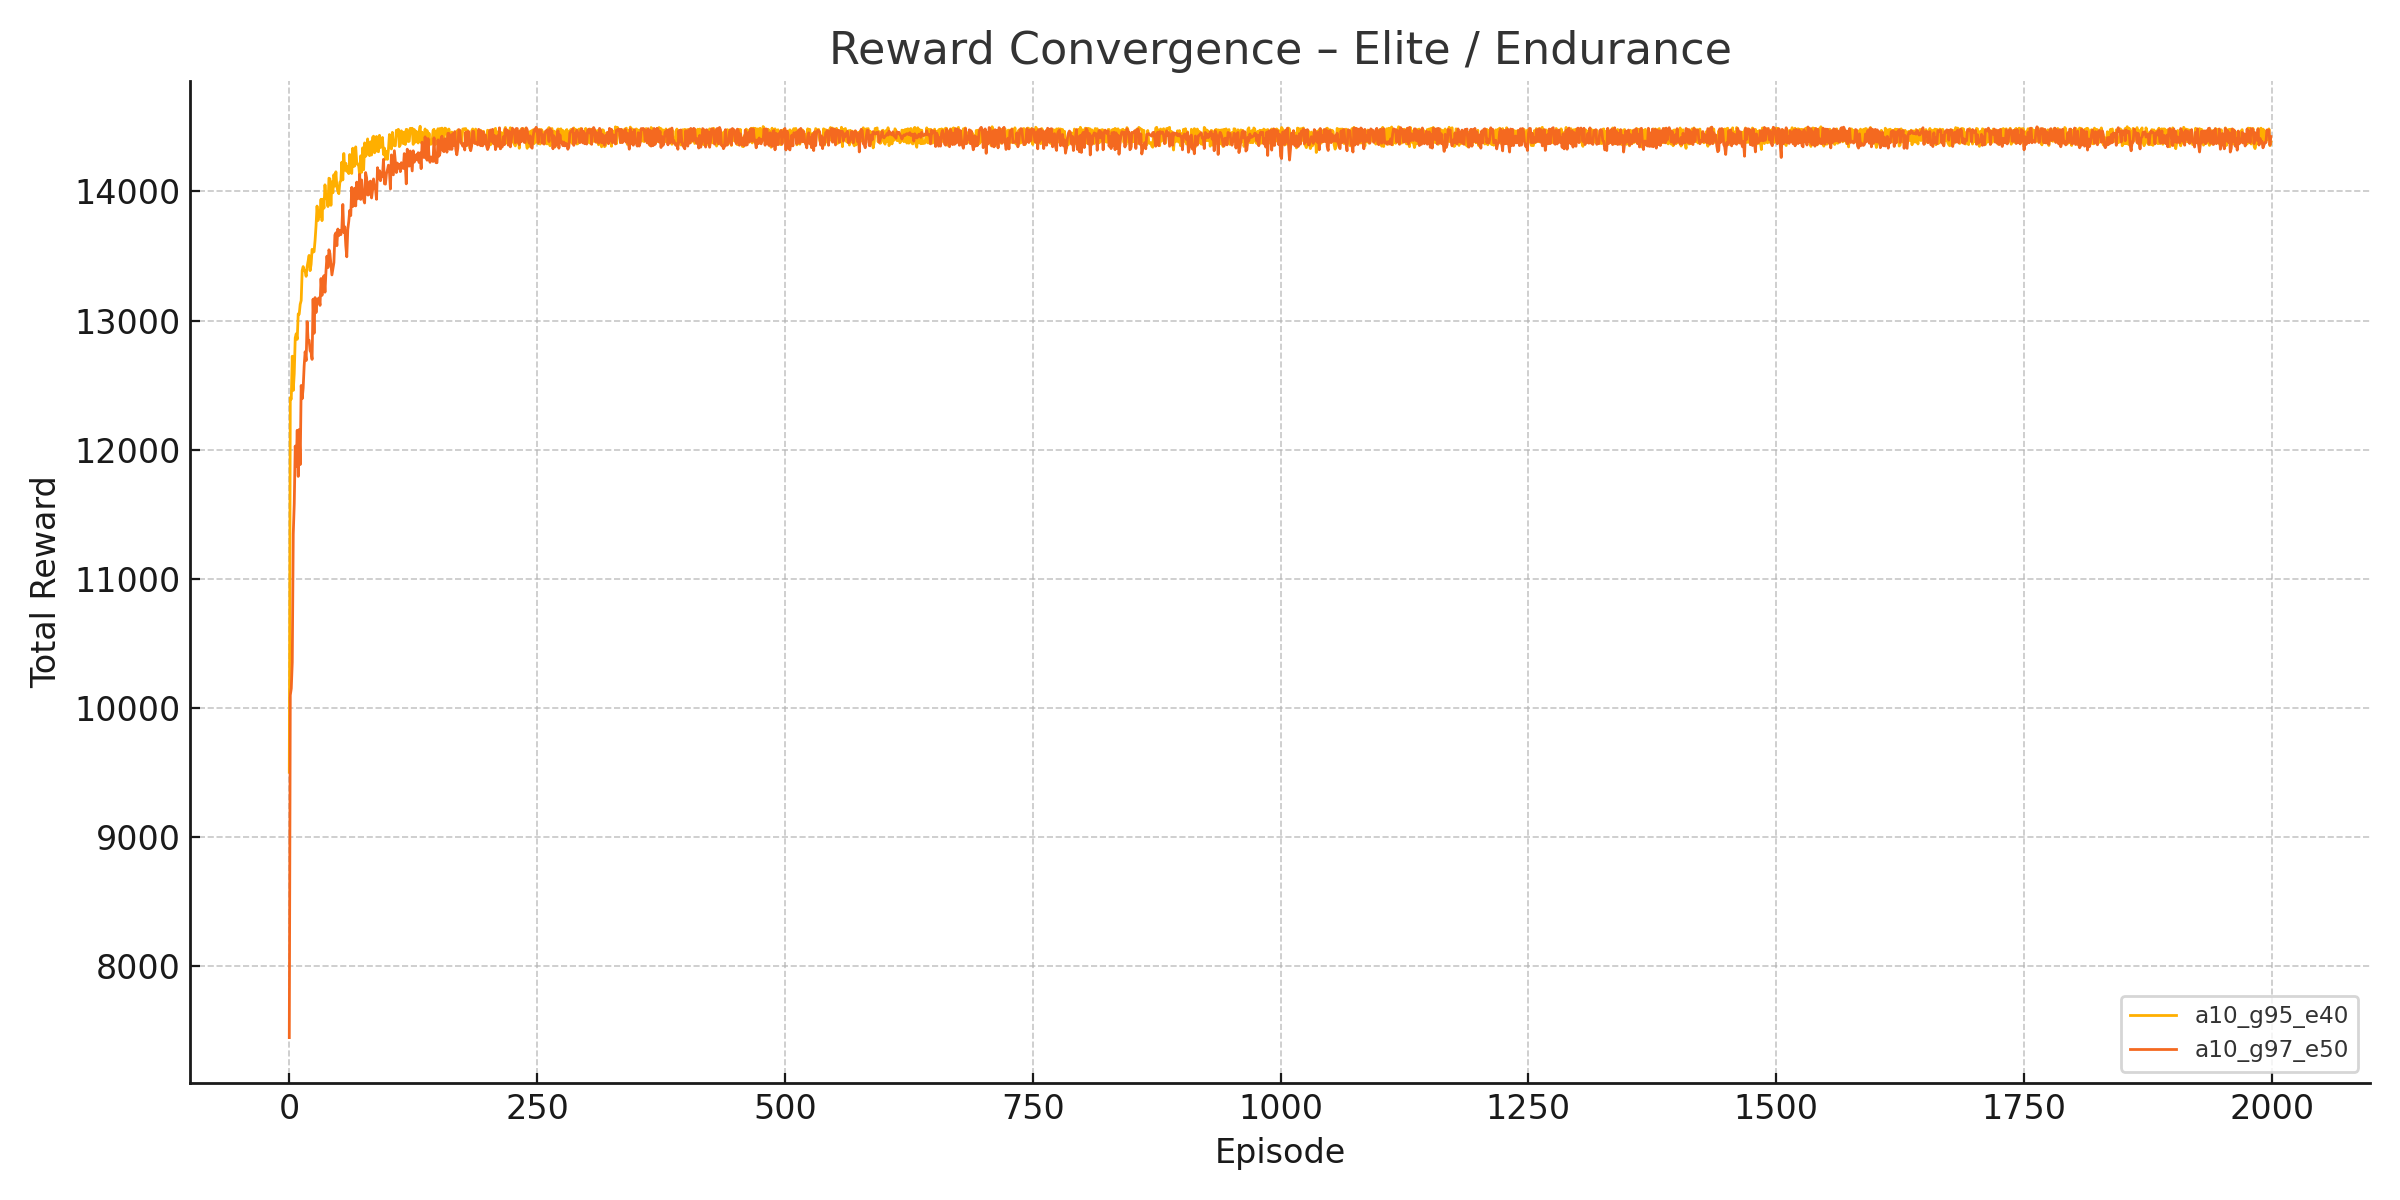
\includegraphics[width=\textwidth]{images/elite_endurance_convergence.png}
    \caption{Endurance}
  \end{subfigure}
  \hfill
  \begin{subfigure}[b]{0.45\textwidth}
    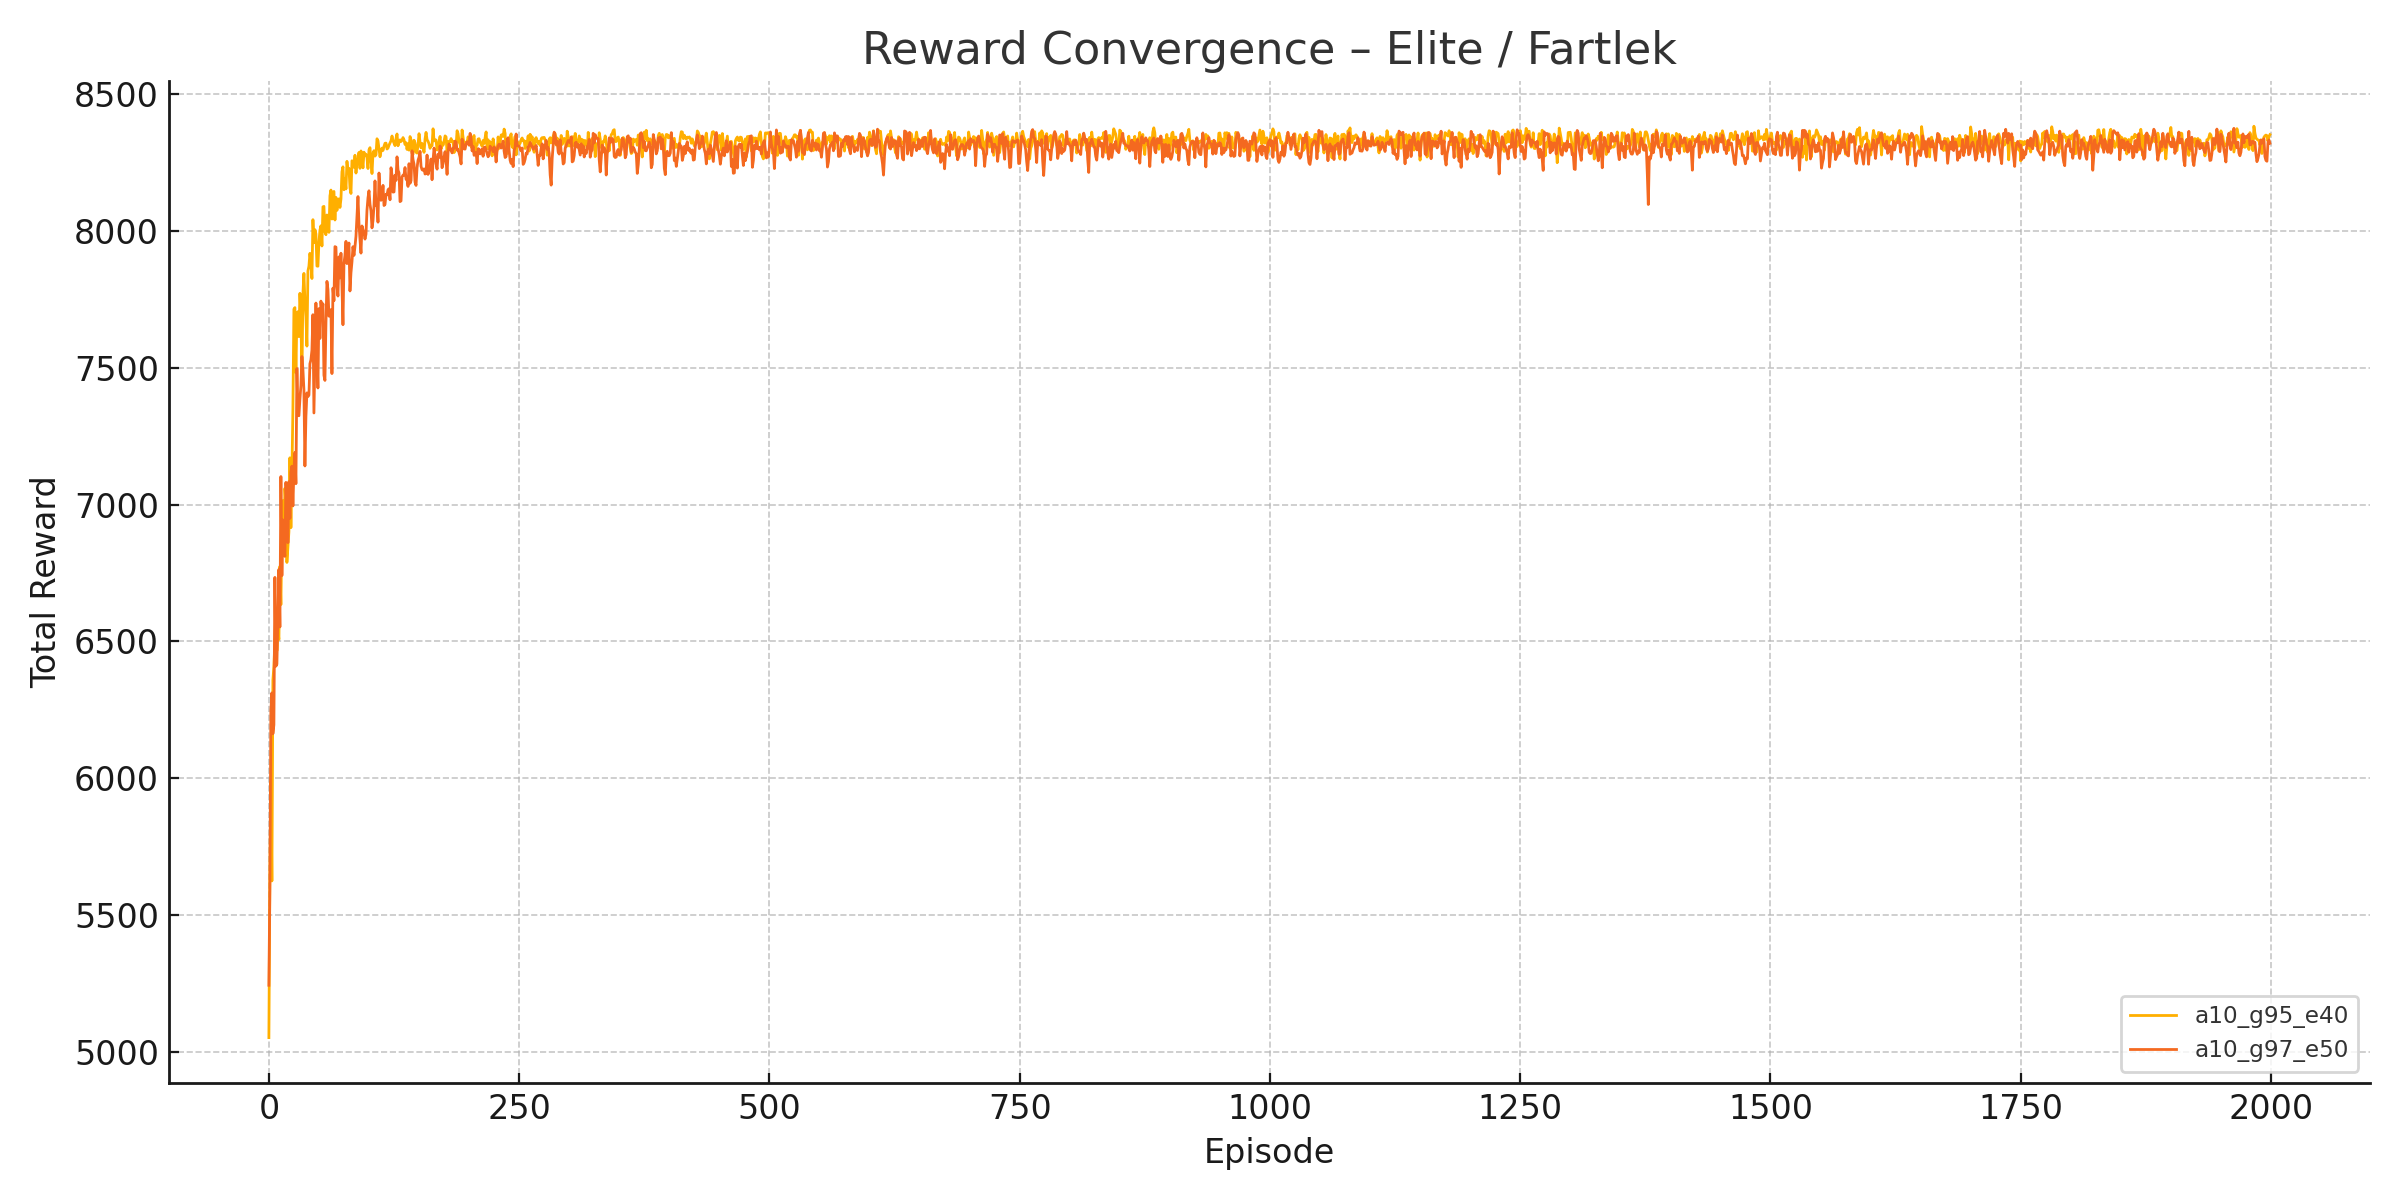
\includegraphics[width=\textwidth]{images/elite_fartlek_convergence.png}
    \caption{Fartlek}
  \end{subfigure}
  \vskip\baselineskip
  \begin{subfigure}[b]{0.45\textwidth}
    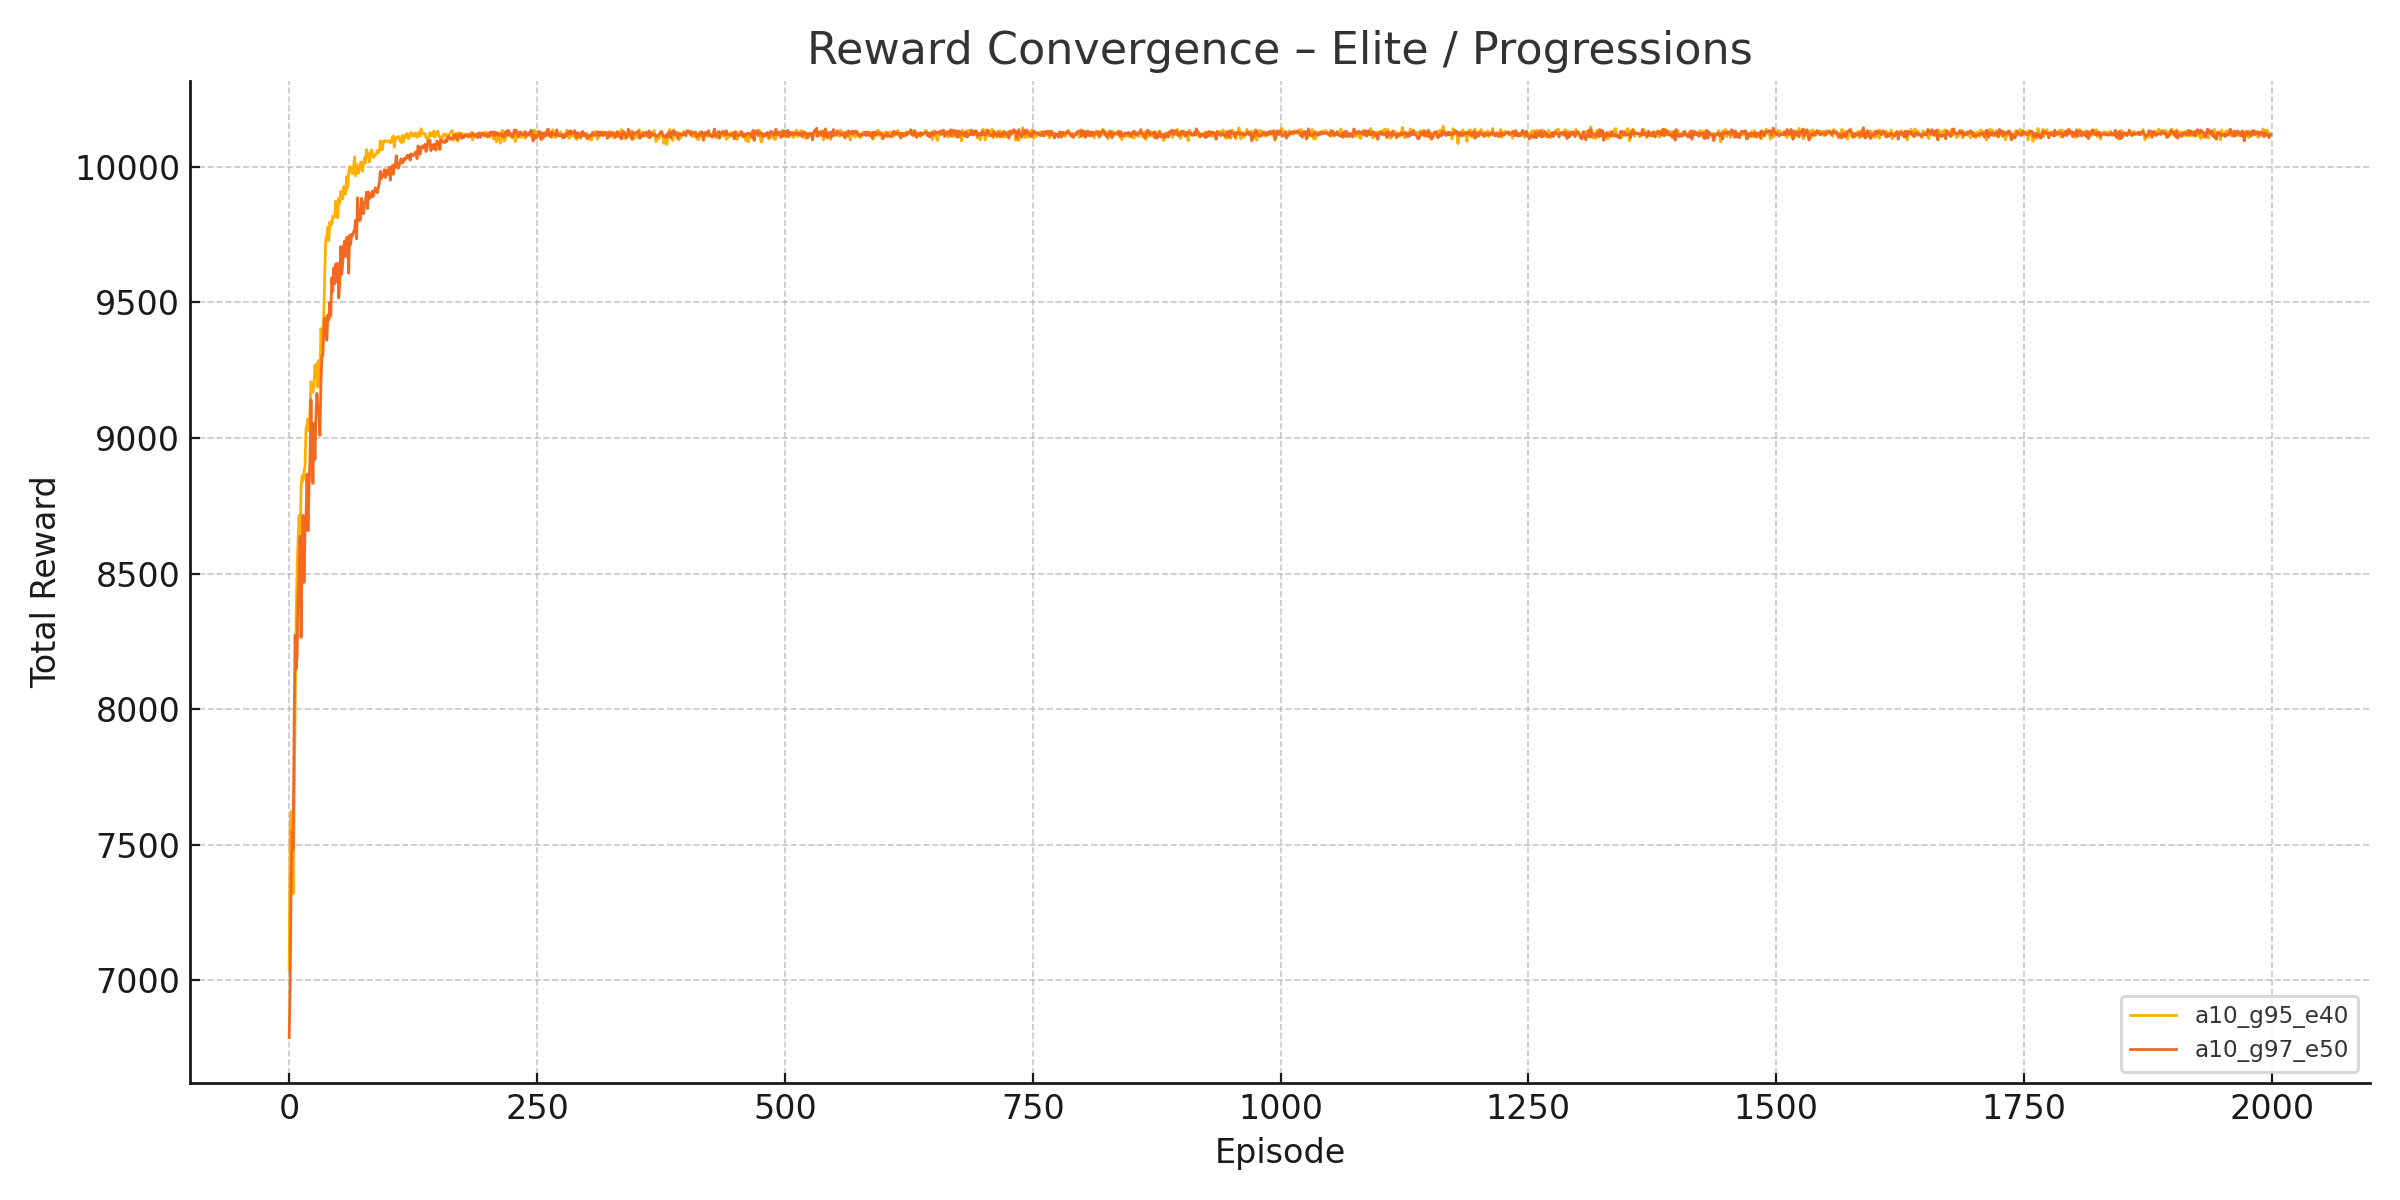
\includegraphics[width=\textwidth]{images/elite_progressions_convergence.png}
    \caption{Progression}
  \end{subfigure}
  \hfill
  \begin{subfigure}[b]{0.45\textwidth}
    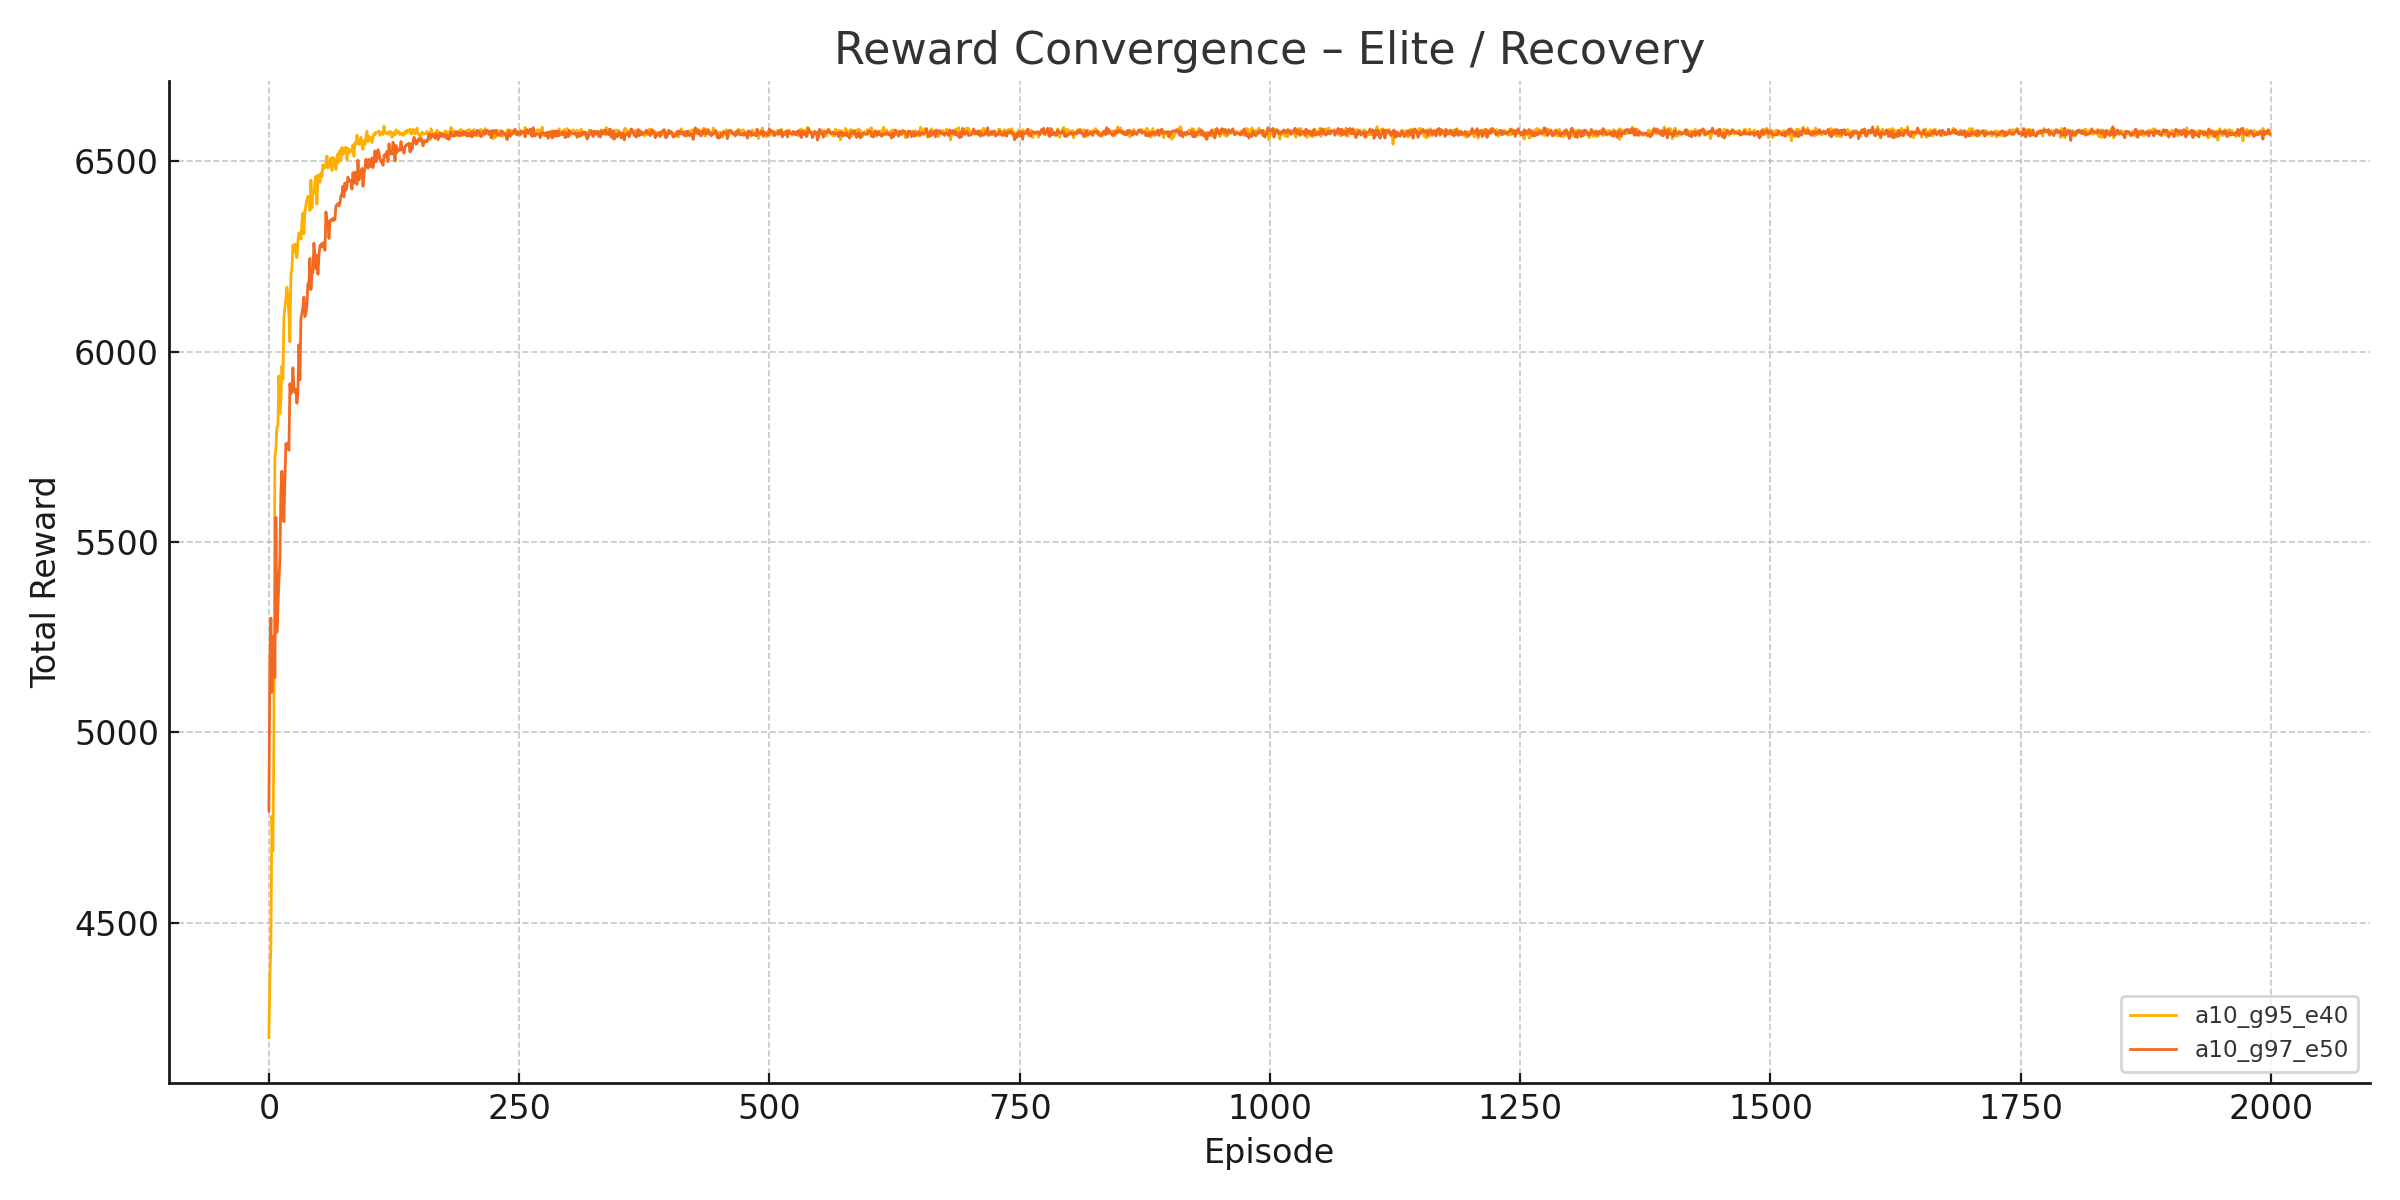
\includegraphics[width=\textwidth]{images/elite_recovery_convergence.png}
    \caption{Recovery}
  \end{subfigure}
  \caption{Reward convergence for \textbf{Elite} (2000 episodes)}
  \label{fig:elite_convergence}
\end{figure}


\begin{figure}[htbp]
  \centering
  \begin{subfigure}[b]{0.45\textwidth}
    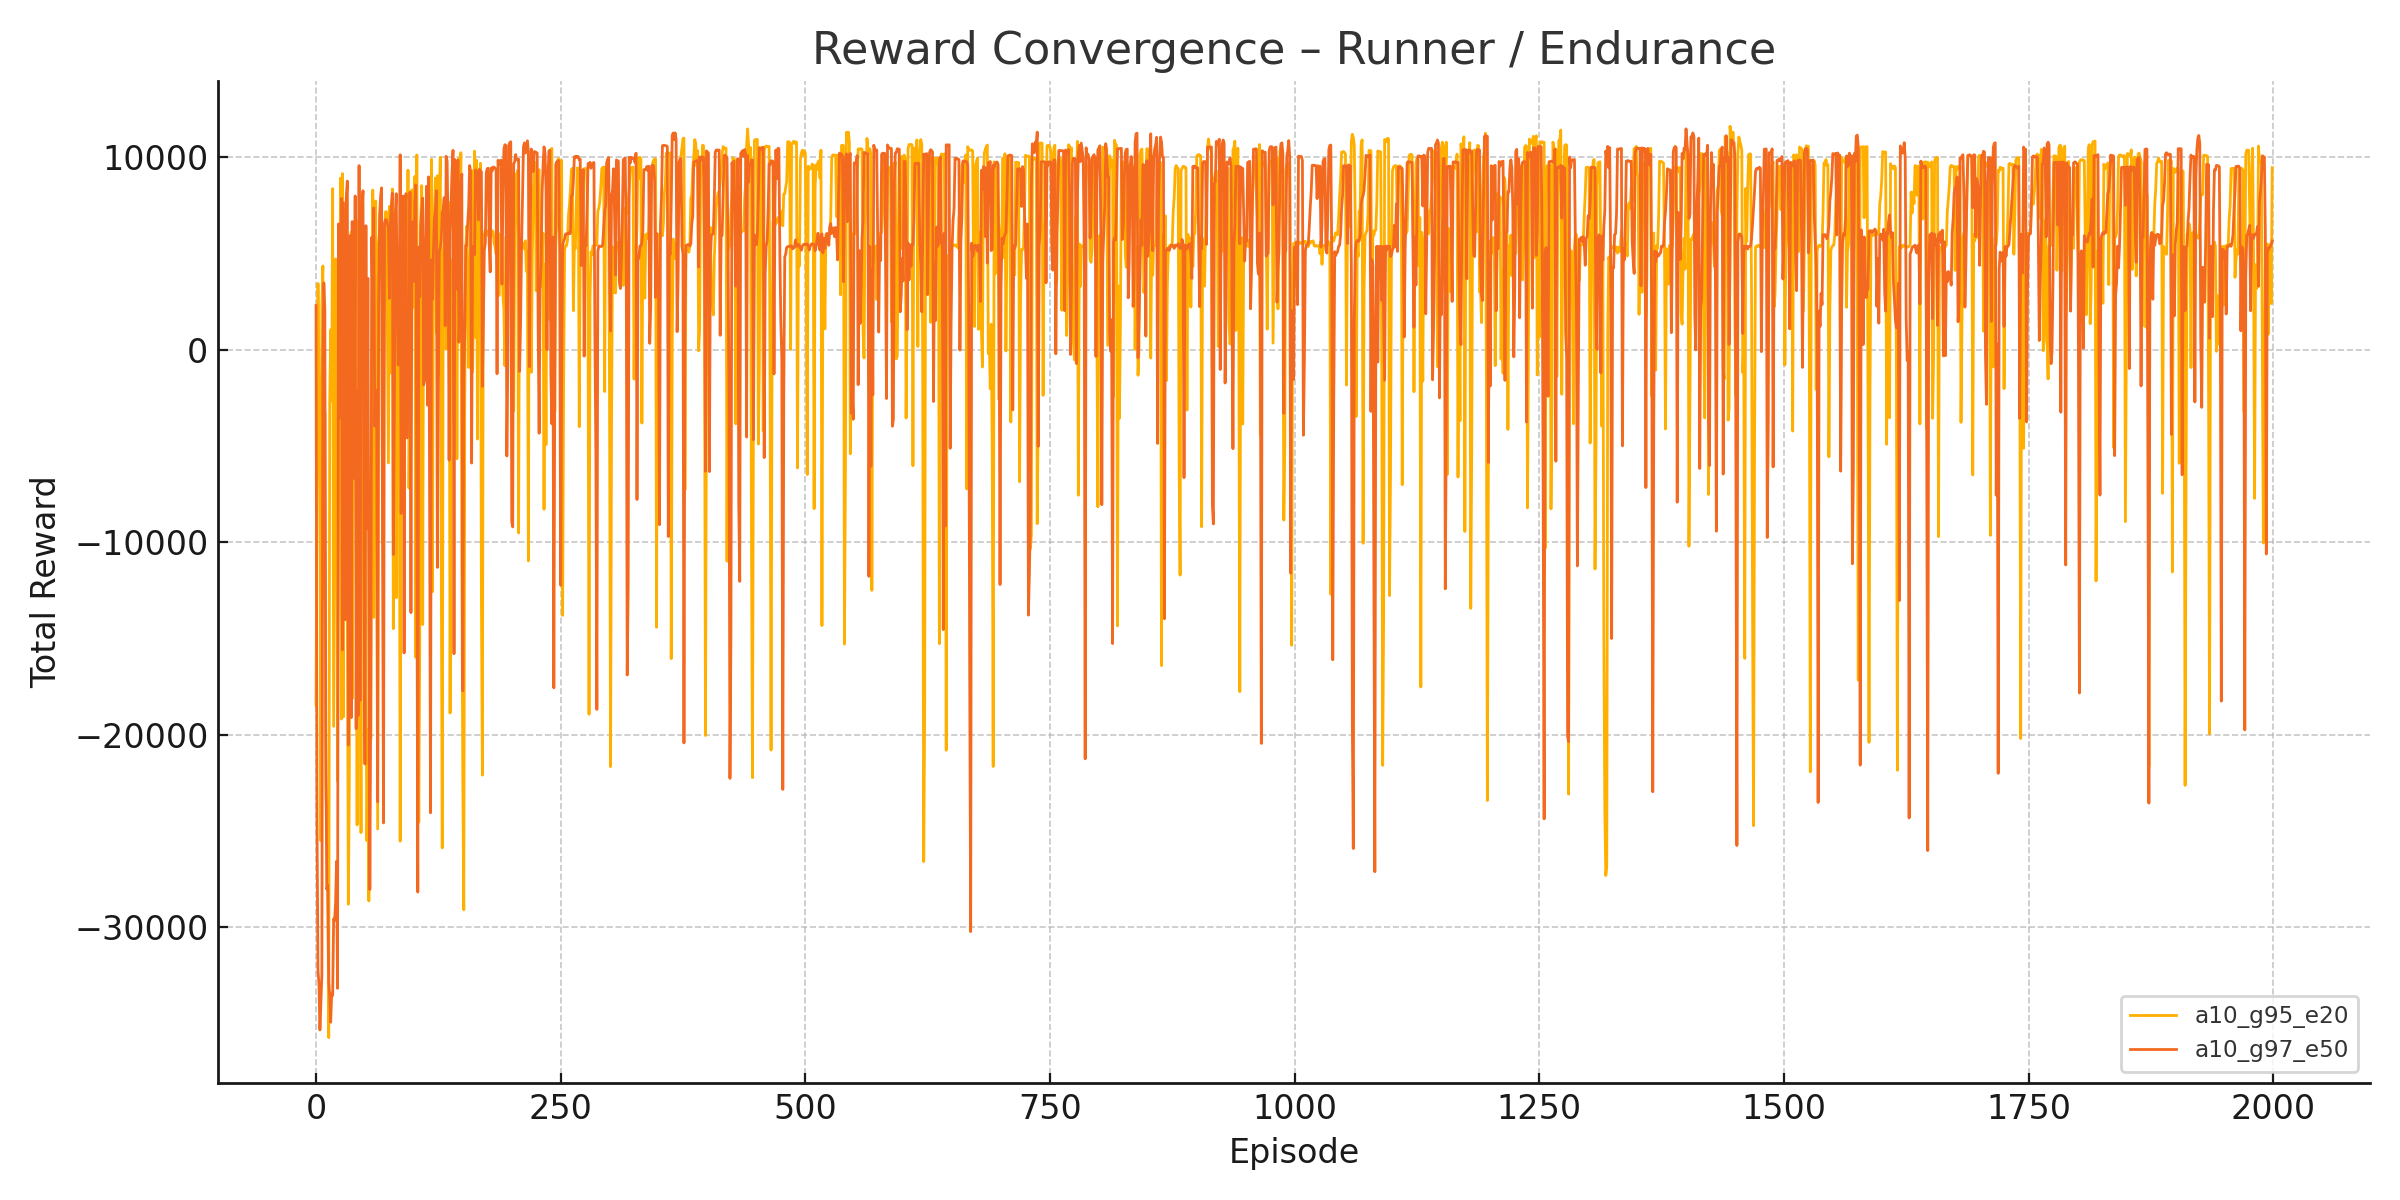
\includegraphics[width=\textwidth]{images/runner_endurance_convergence.png}
    \caption{Endurance}
  \end{subfigure}
  \hfill
  \begin{subfigure}[b]{0.45\textwidth}
    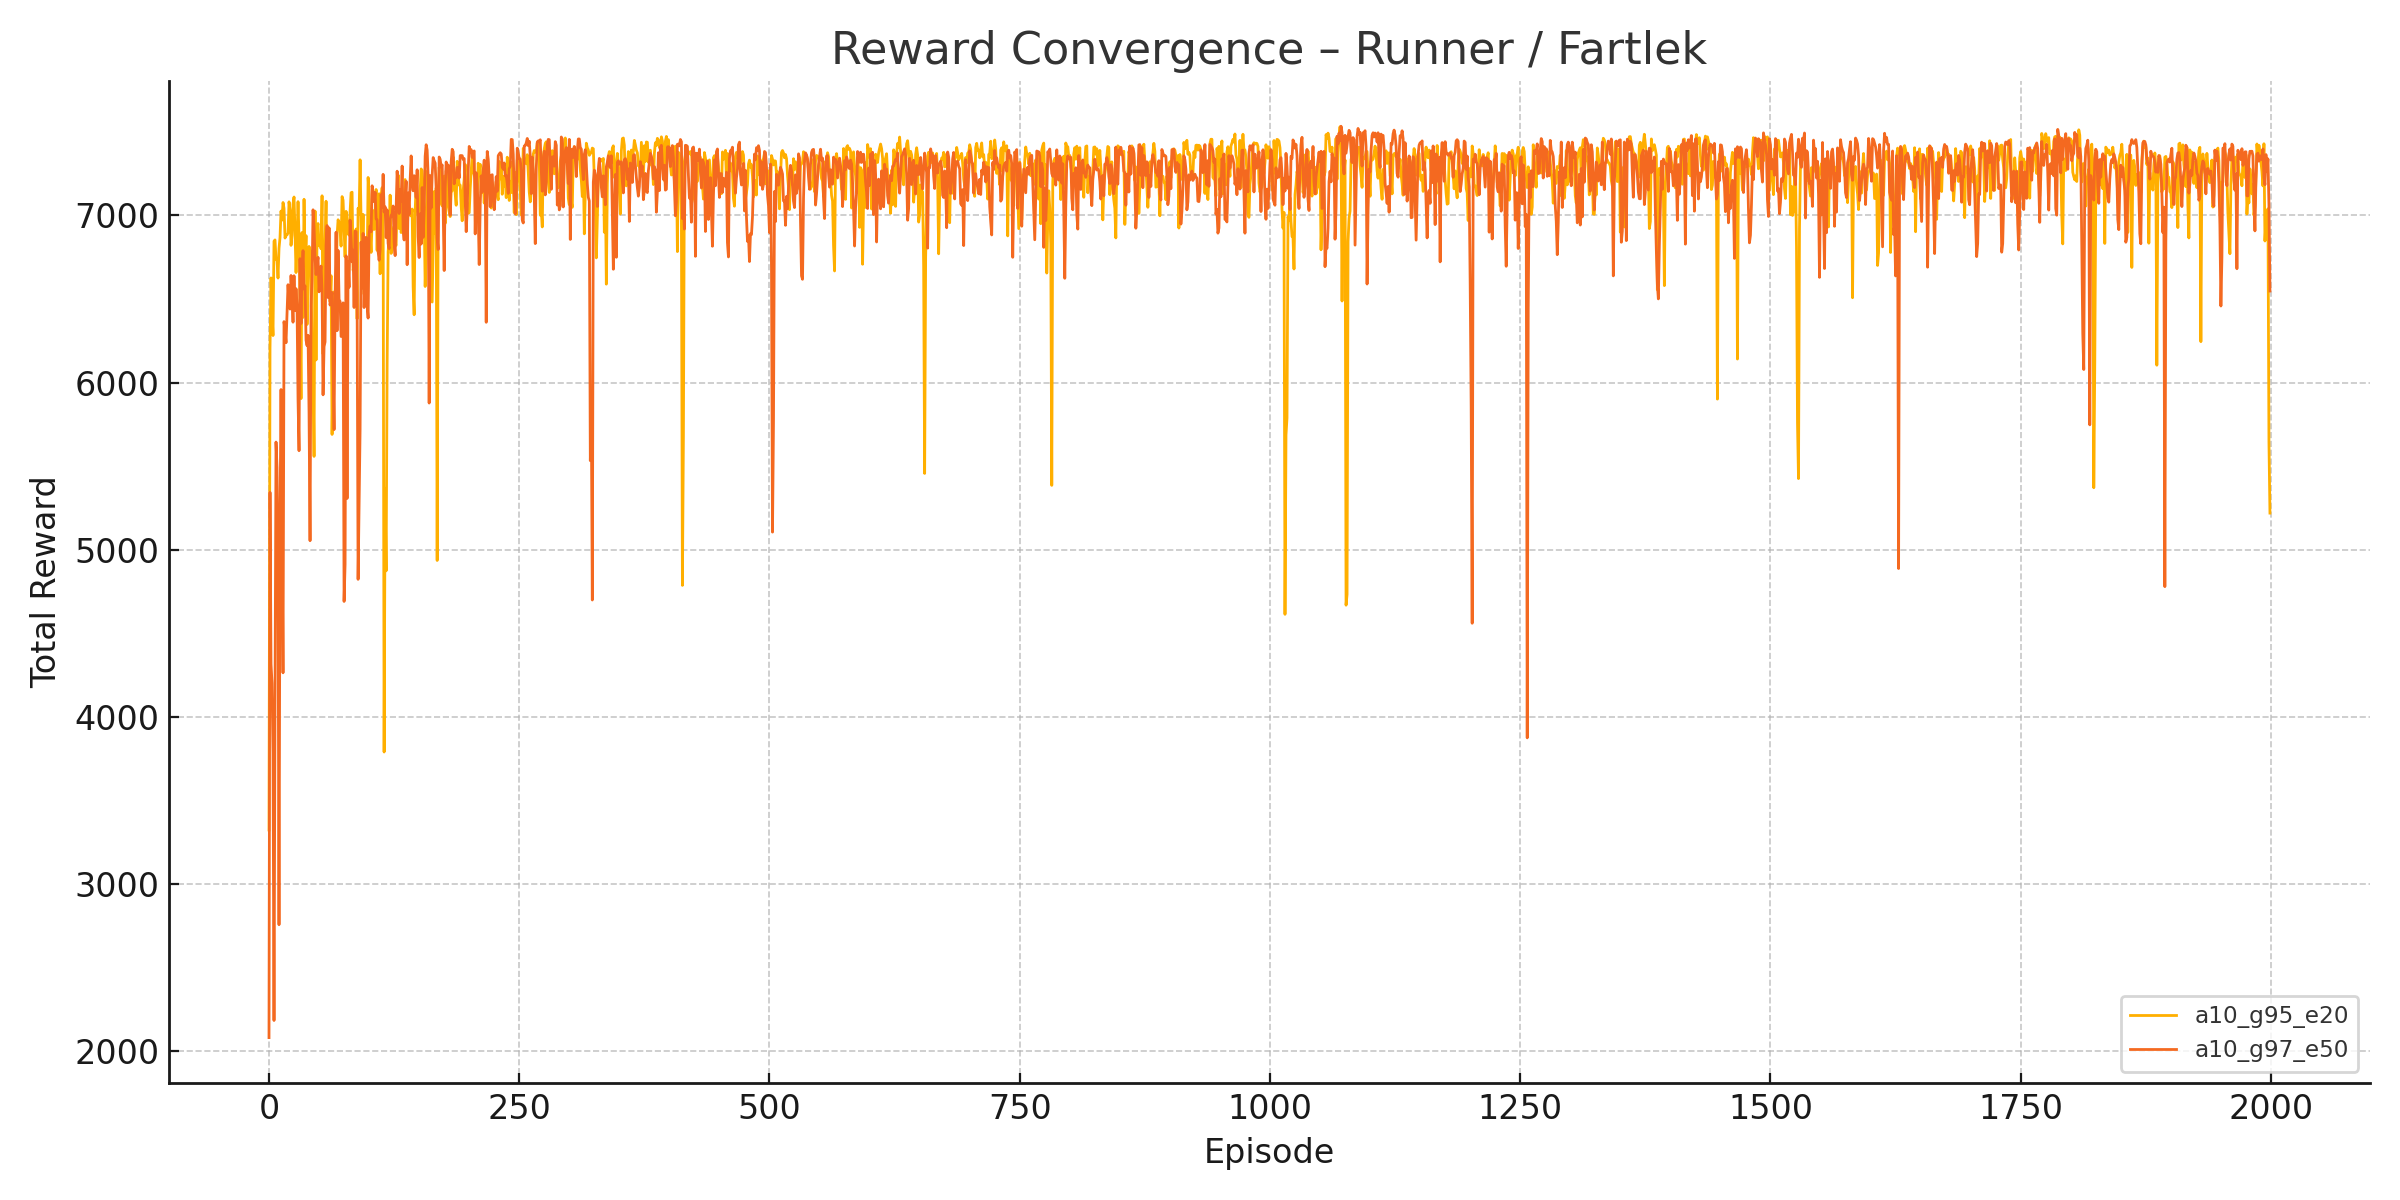
\includegraphics[width=\textwidth]{images/runner_fartlek_convergence.png}
    \caption{Fartlek}
  \end{subfigure}
  \vskip\baselineskip
  \begin{subfigure}[b]{0.45\textwidth}
    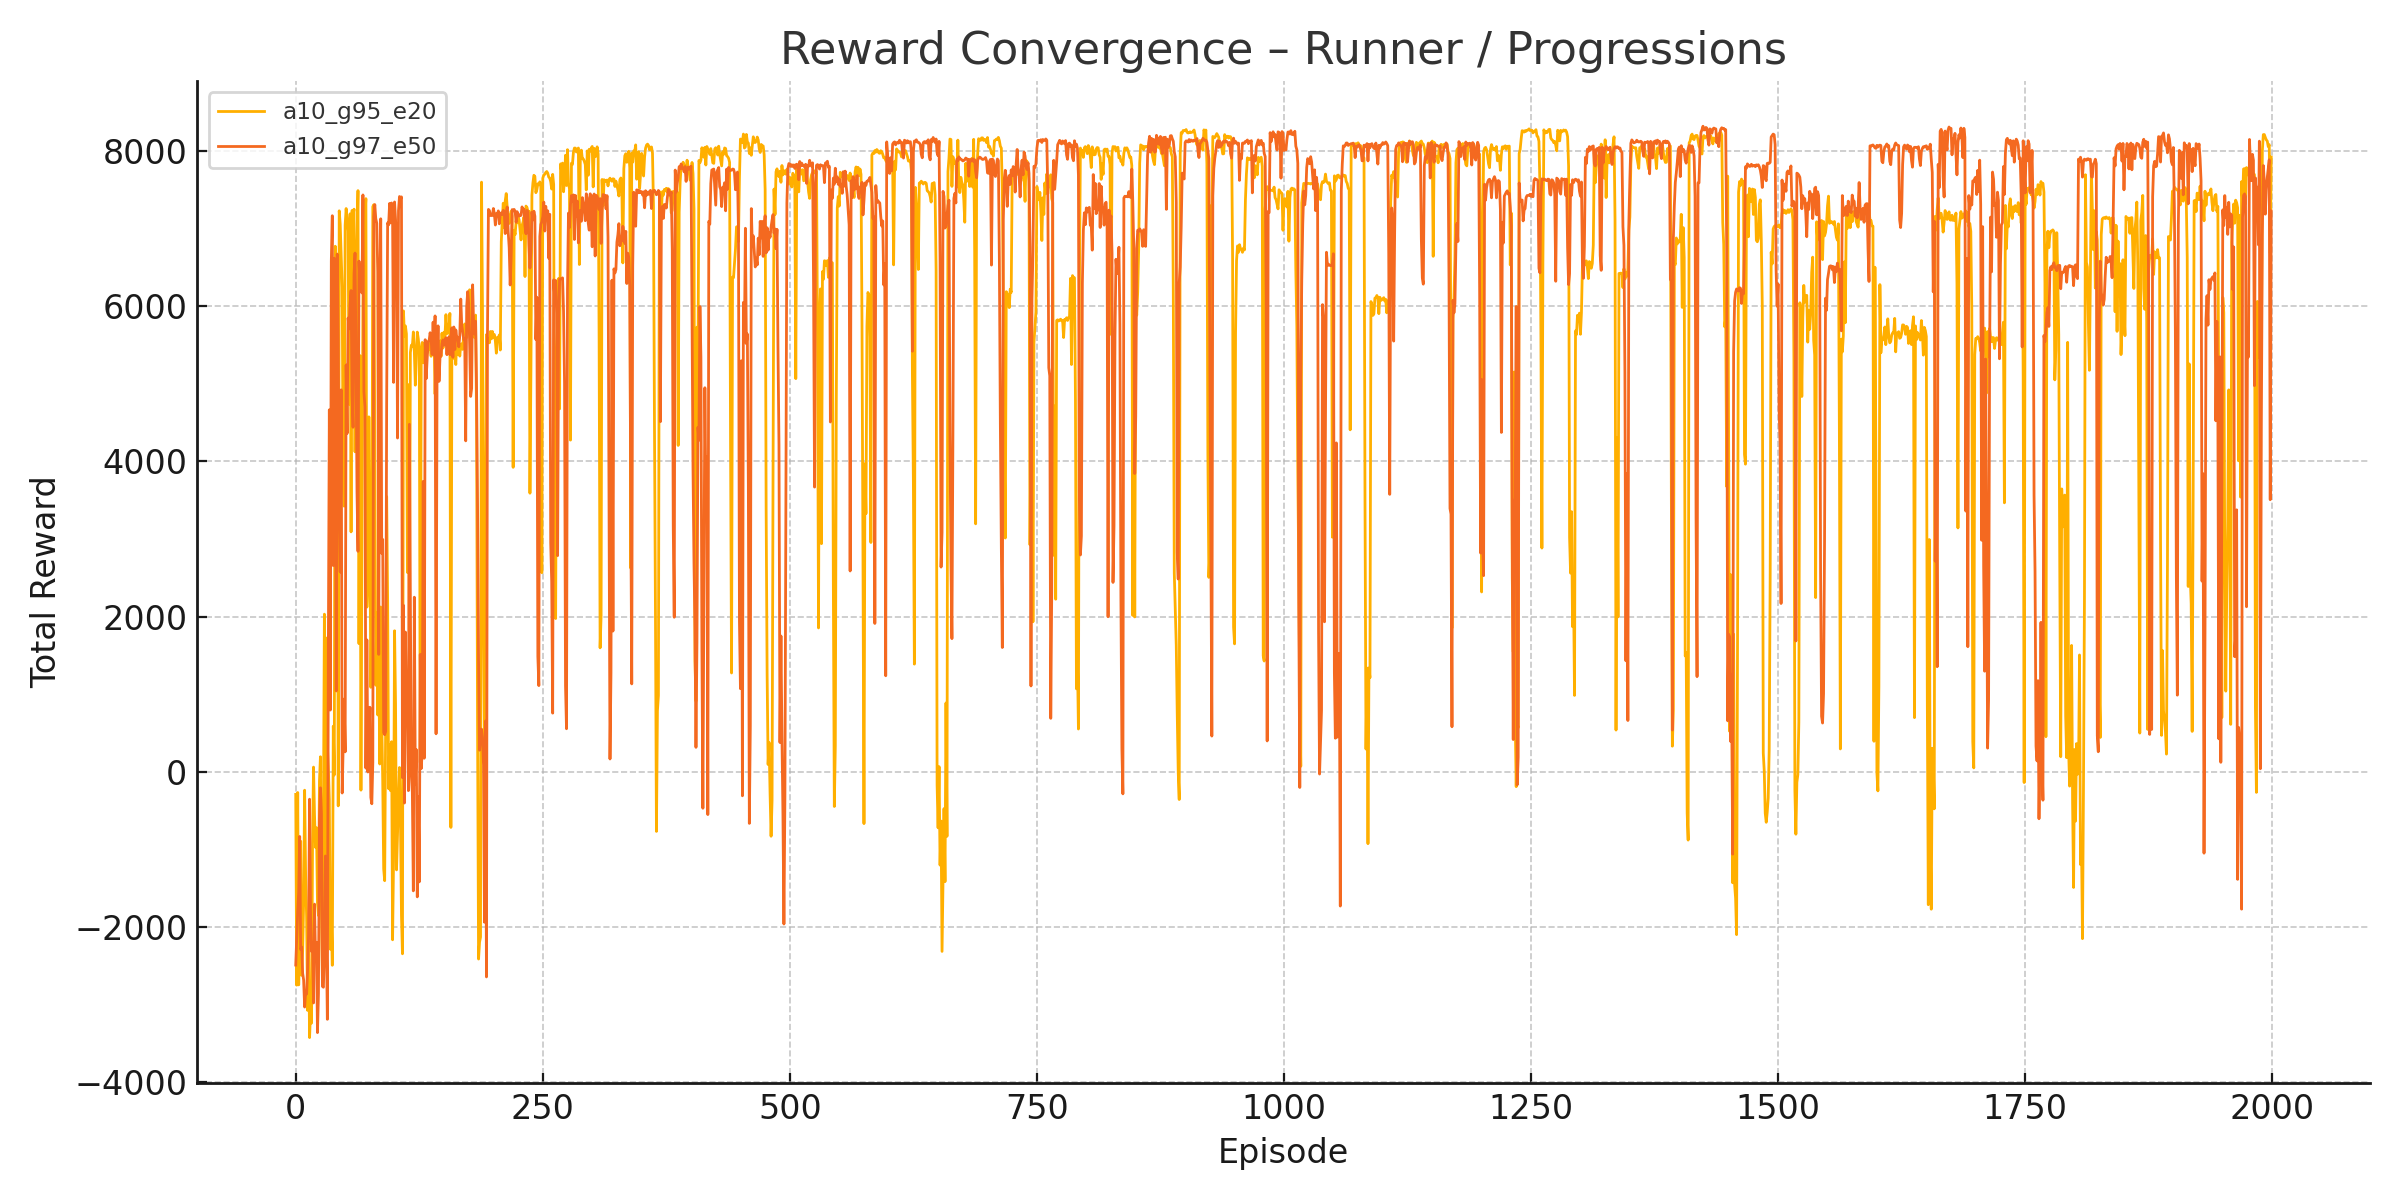
\includegraphics[width=\textwidth]{images/runner_progressions_convergence.png}
    \caption{Progression}
  \end{subfigure}
  \hfill
  \begin{subfigure}[b]{0.45\textwidth}
    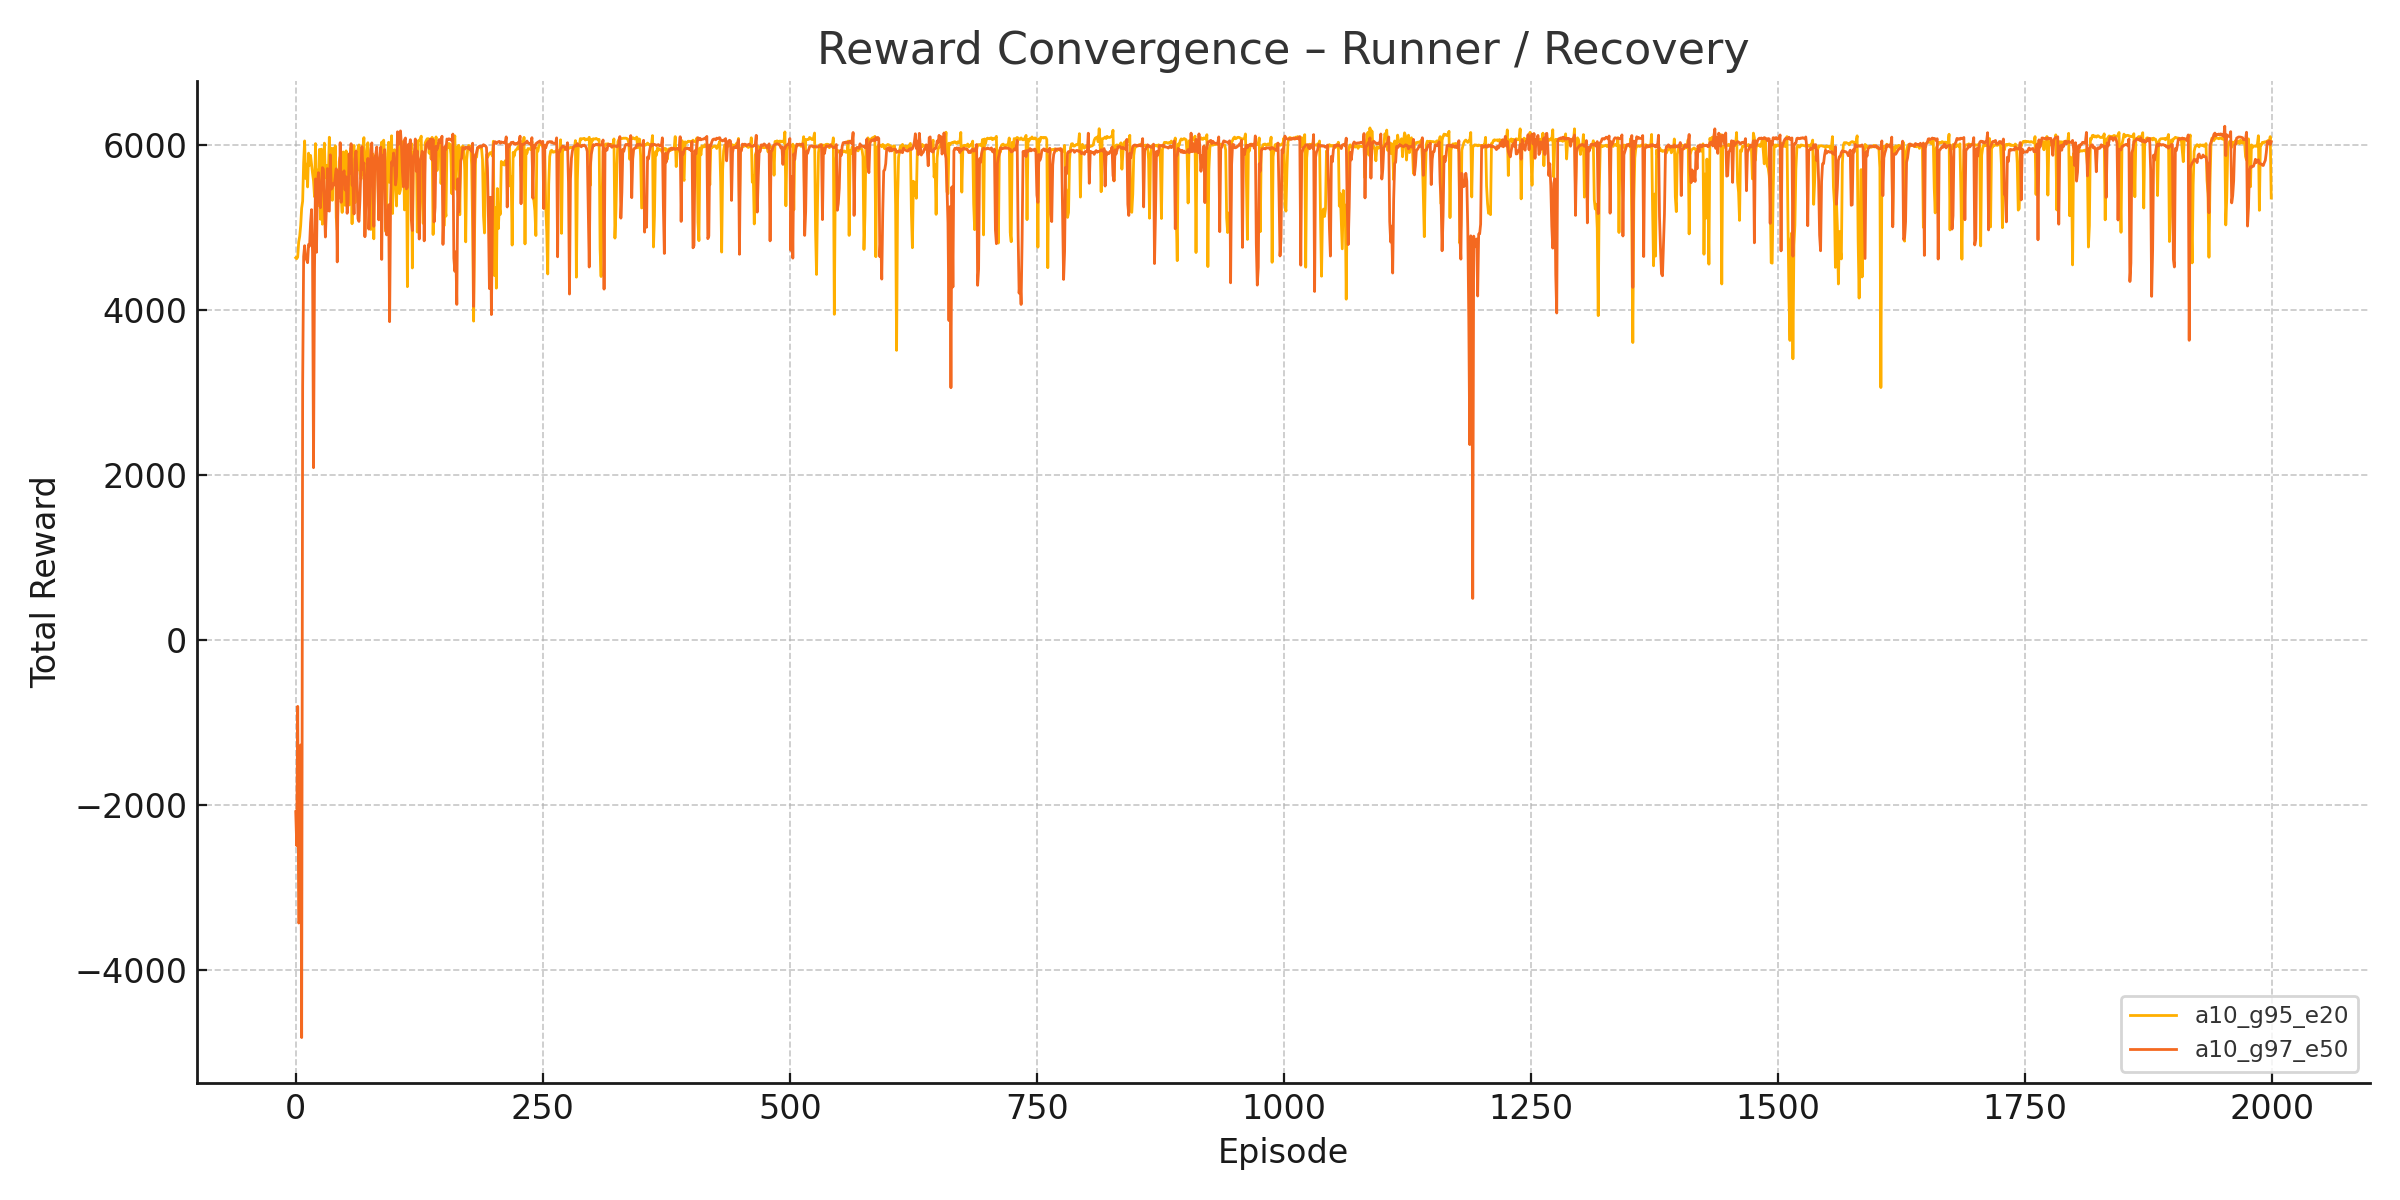
\includegraphics[width=\textwidth]{images/runner_recovery_convergence.png}
    \caption{Recovery}
  \end{subfigure}
  \caption{Reward convergence for \textbf{Runner} (2000 episodes)}
  \label{fig:runner_convergence}
\end{figure}


\begin{figure}[htbp]
  \centering
  \begin{subfigure}[b]{0.45\textwidth}
    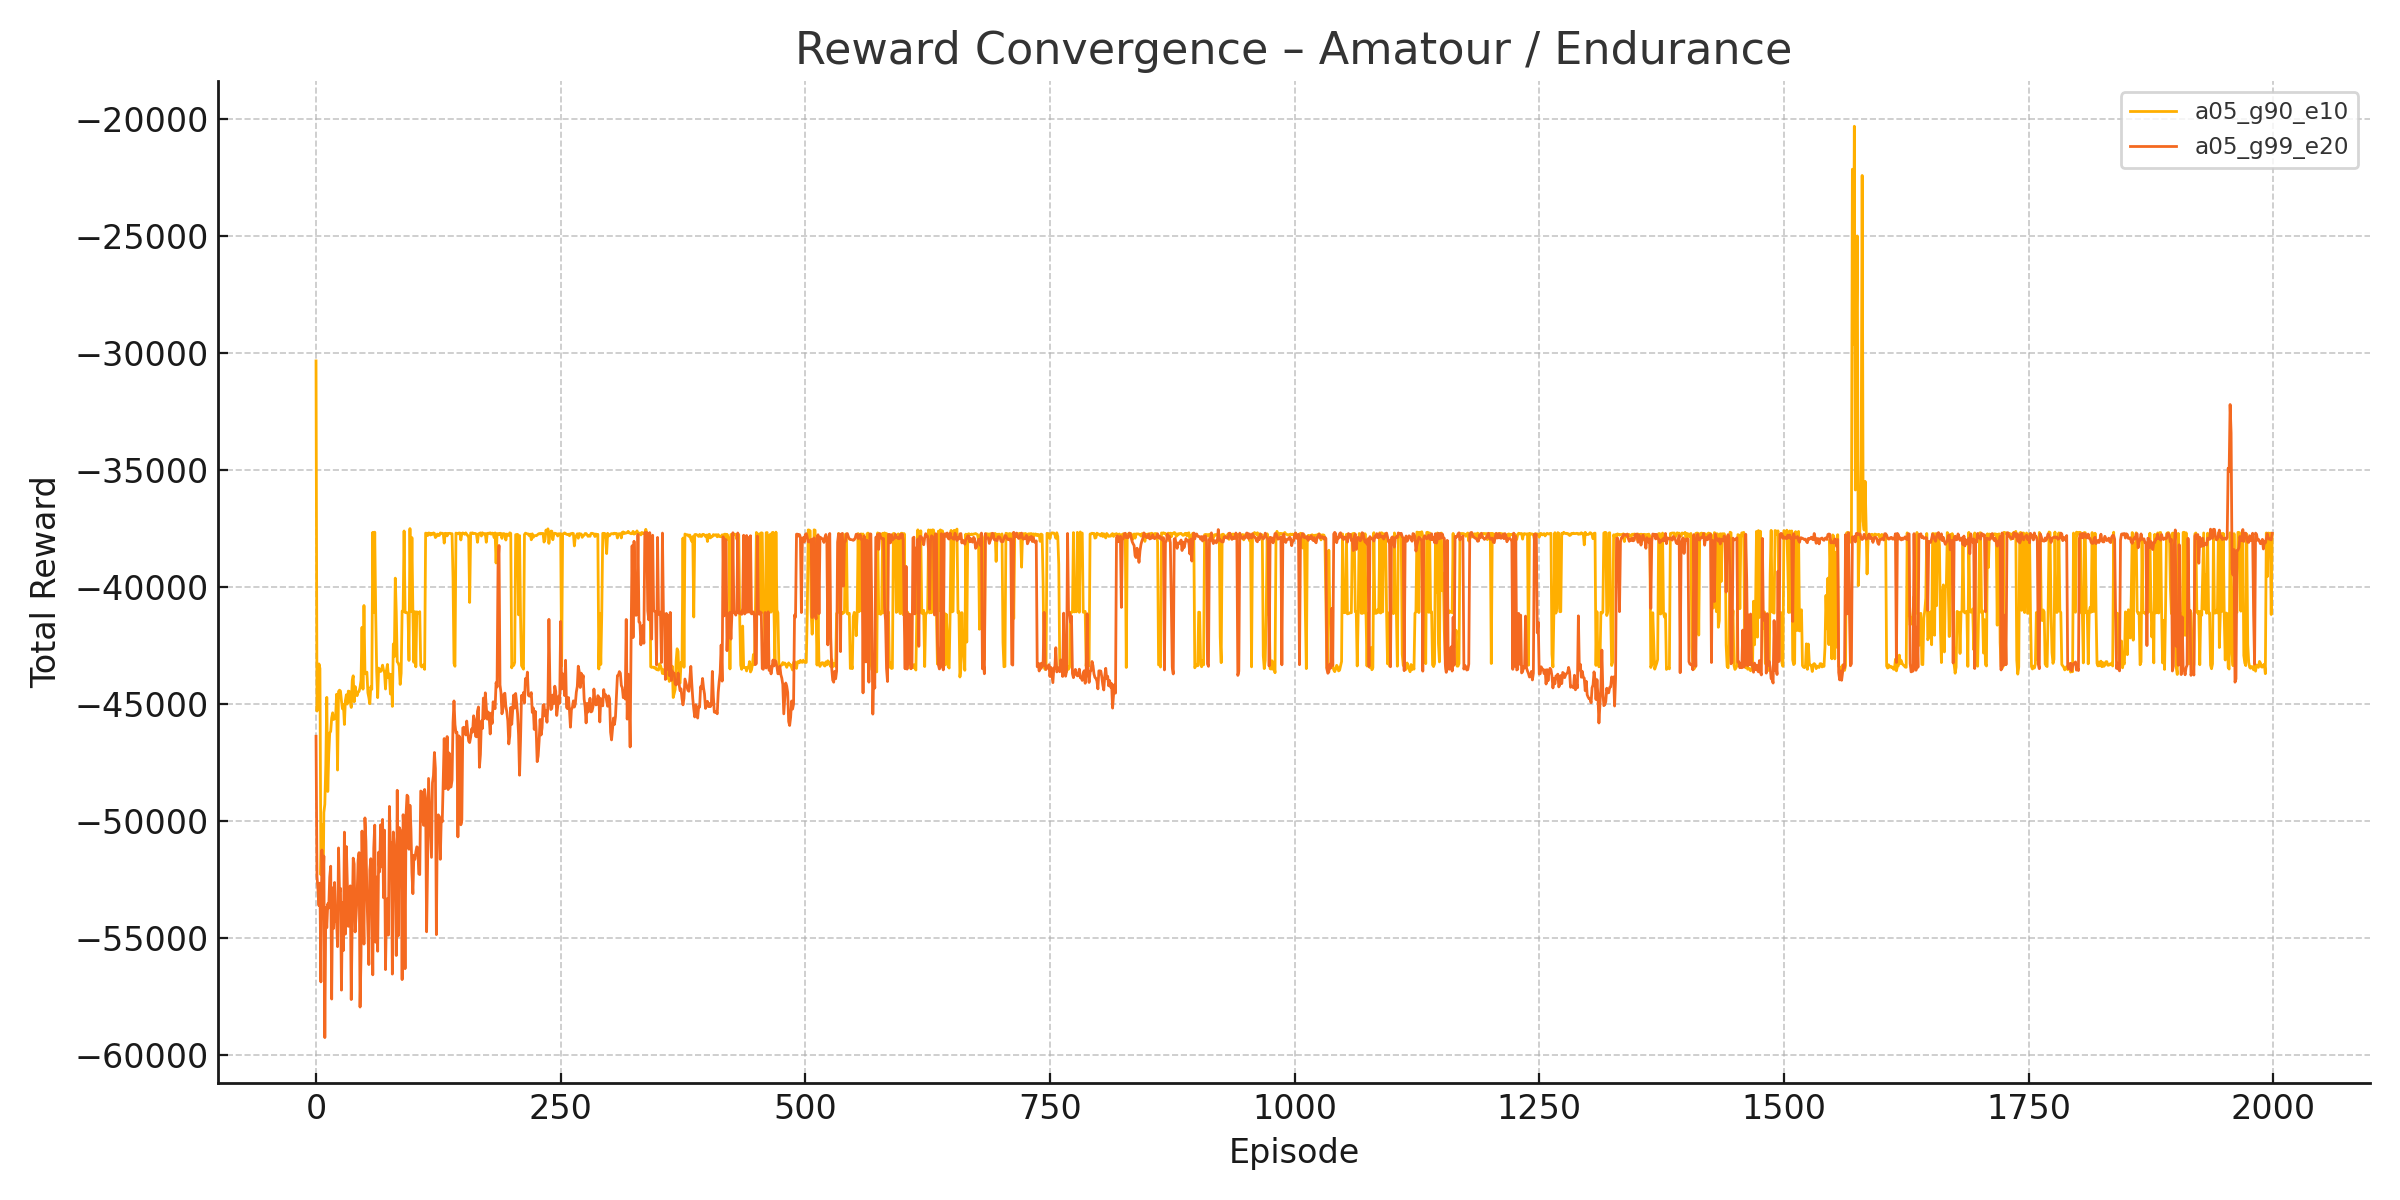
\includegraphics[width=\textwidth]{images/amatour_endurance_convergence.png}
    \caption{Endurance}
  \end{subfigure}
  \hfill
  \begin{subfigure}[b]{0.45\textwidth}
    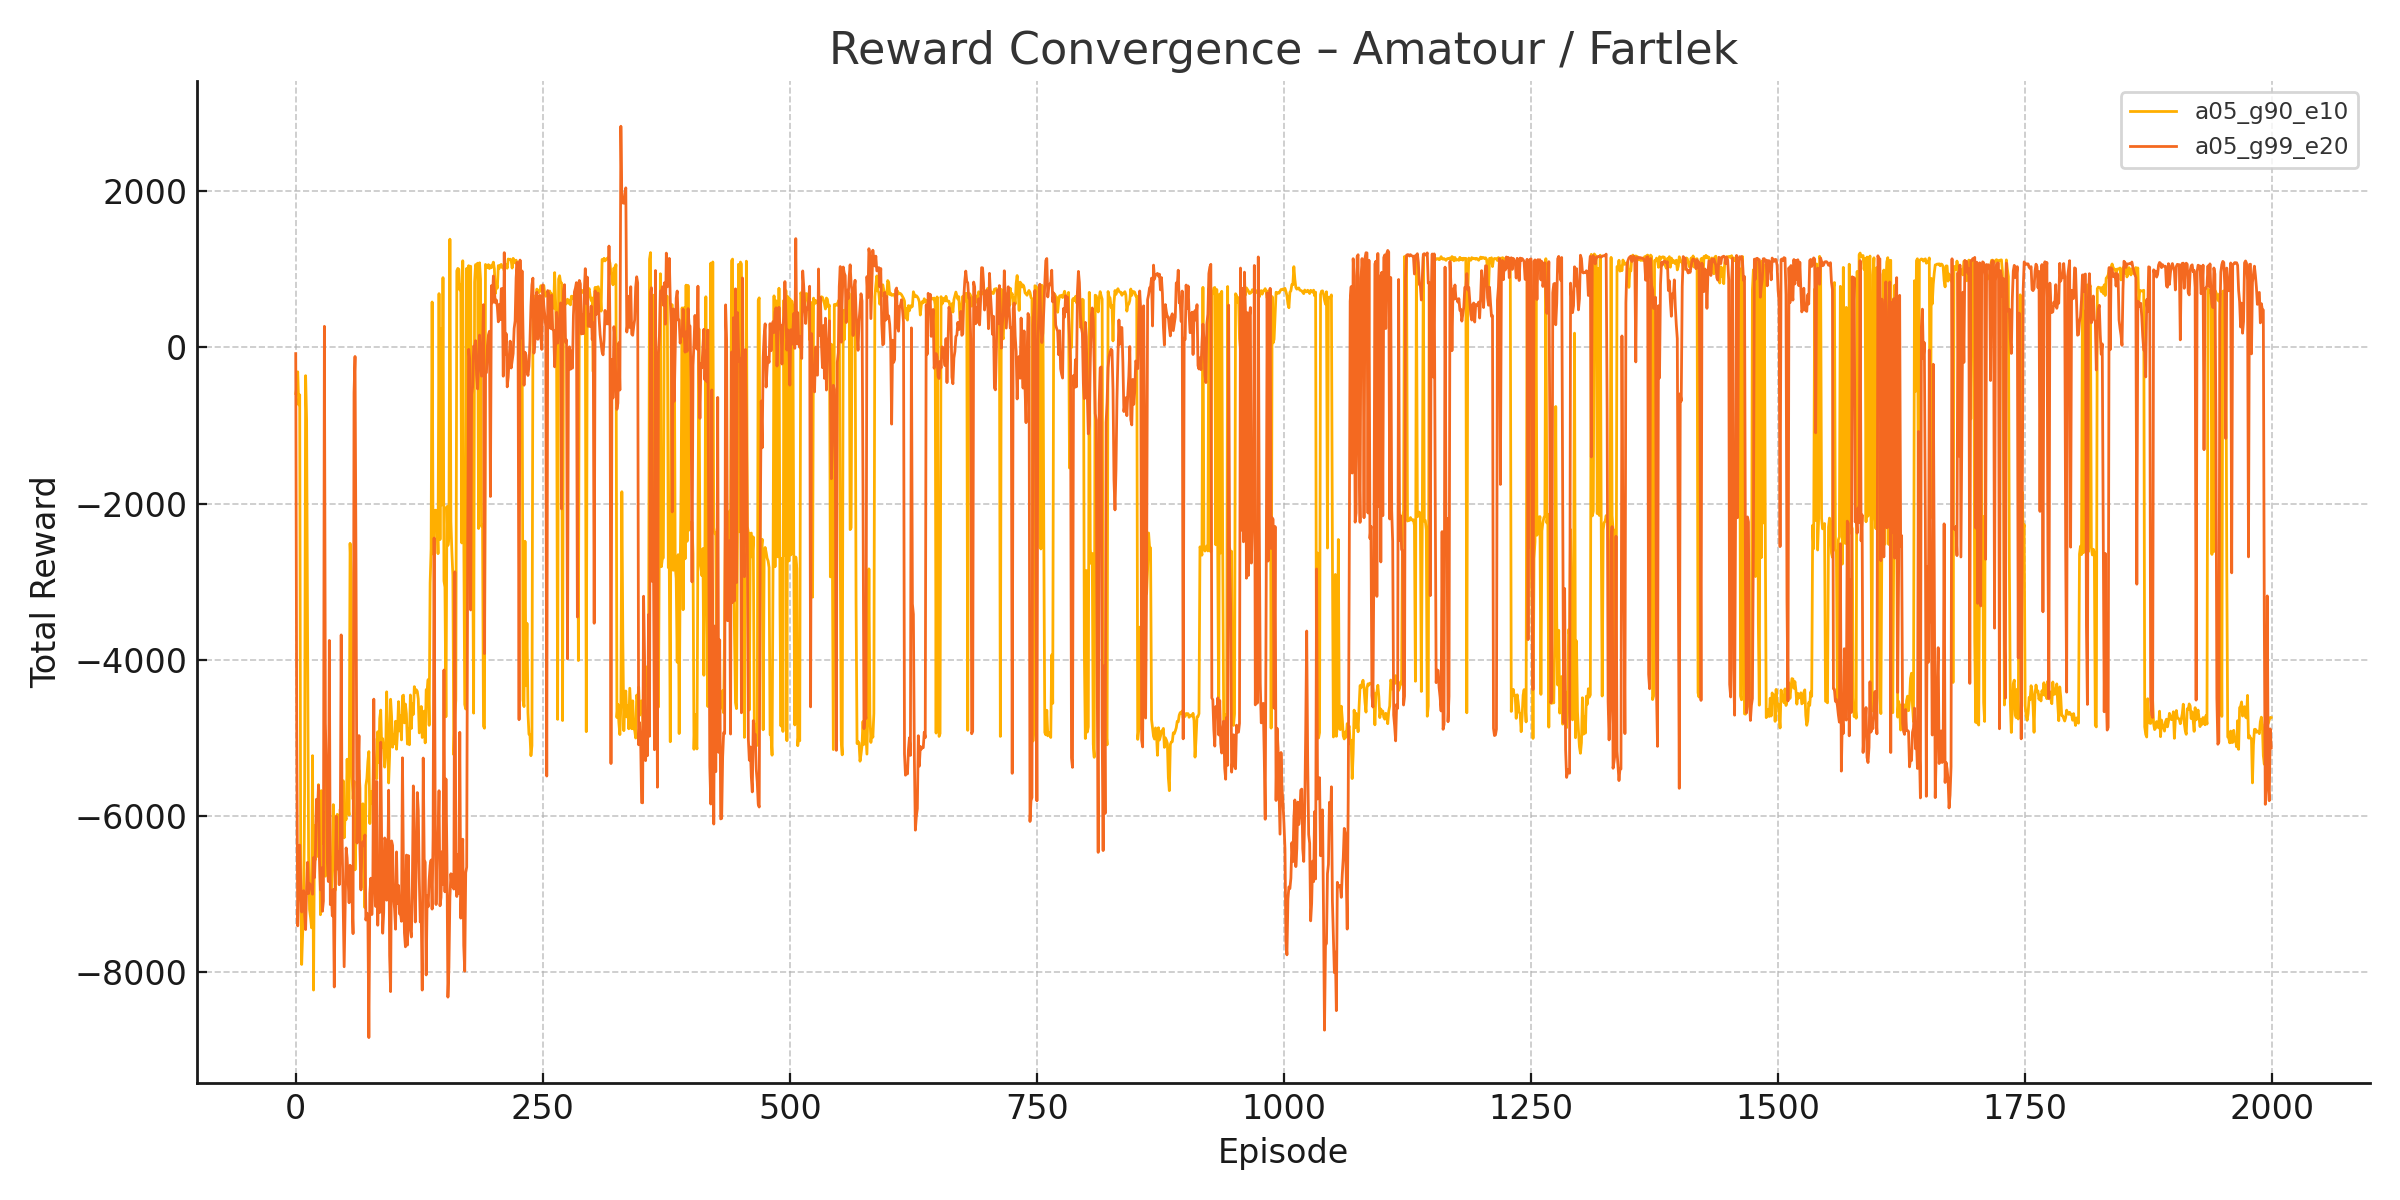
\includegraphics[width=\textwidth]{images/amatour_fartlek_convergence.png}
    \caption{Fartlek}
  \end{subfigure}
  \vskip\baselineskip
  \begin{subfigure}[b]{0.45\textwidth}
    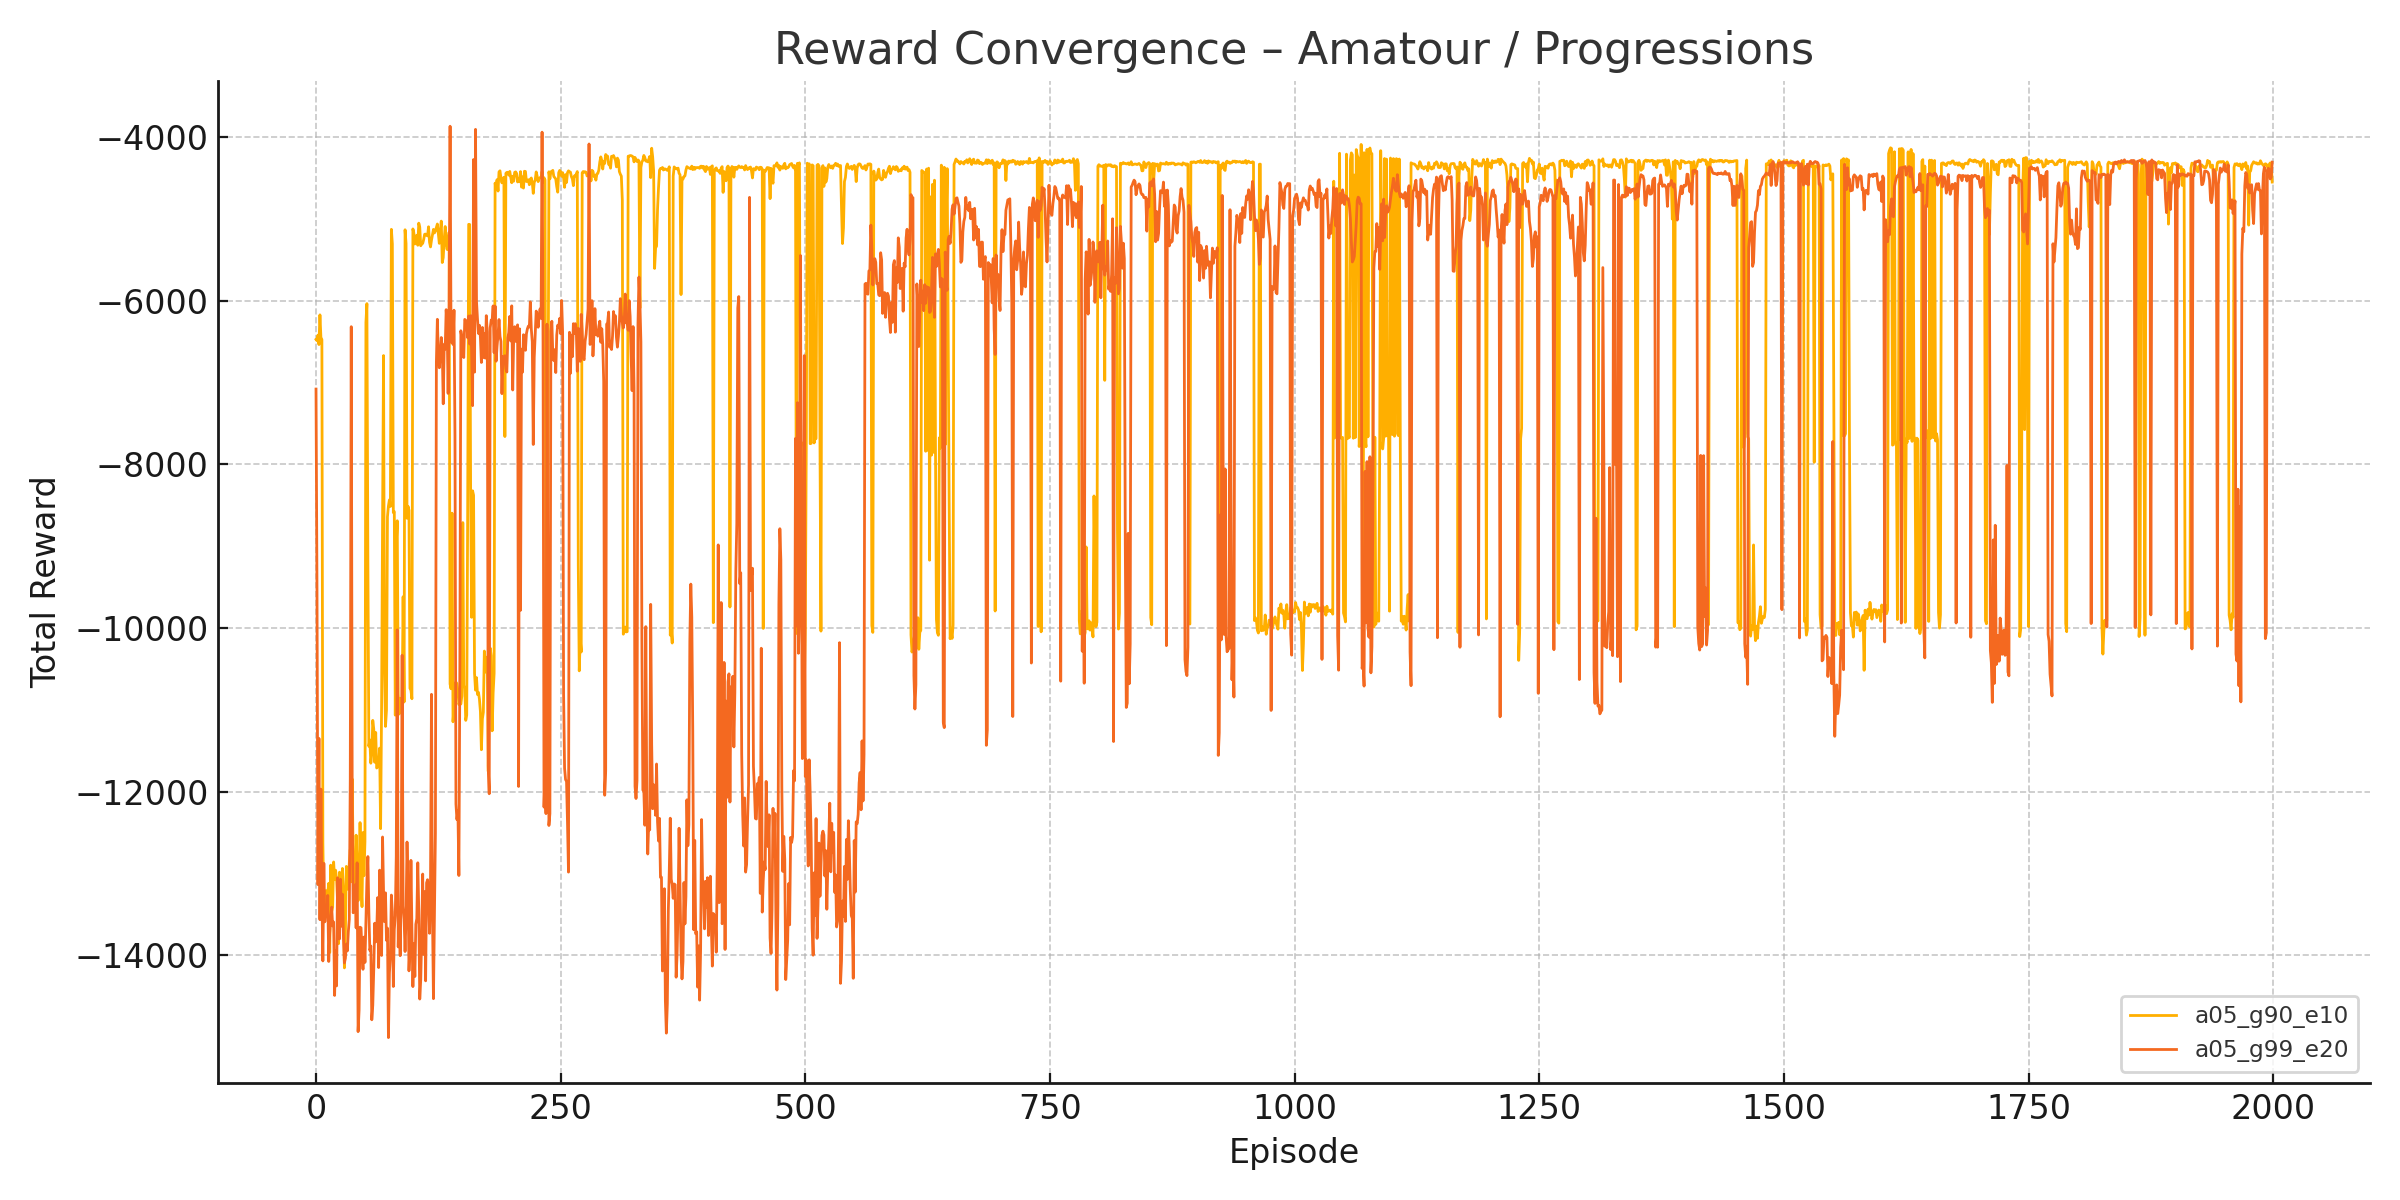
\includegraphics[width=\textwidth]{images/amatour_progressions_convergence.png}
    \caption{Progression}
  \end{subfigure}
  \hfill
  \begin{subfigure}[b]{0.45\textwidth}
    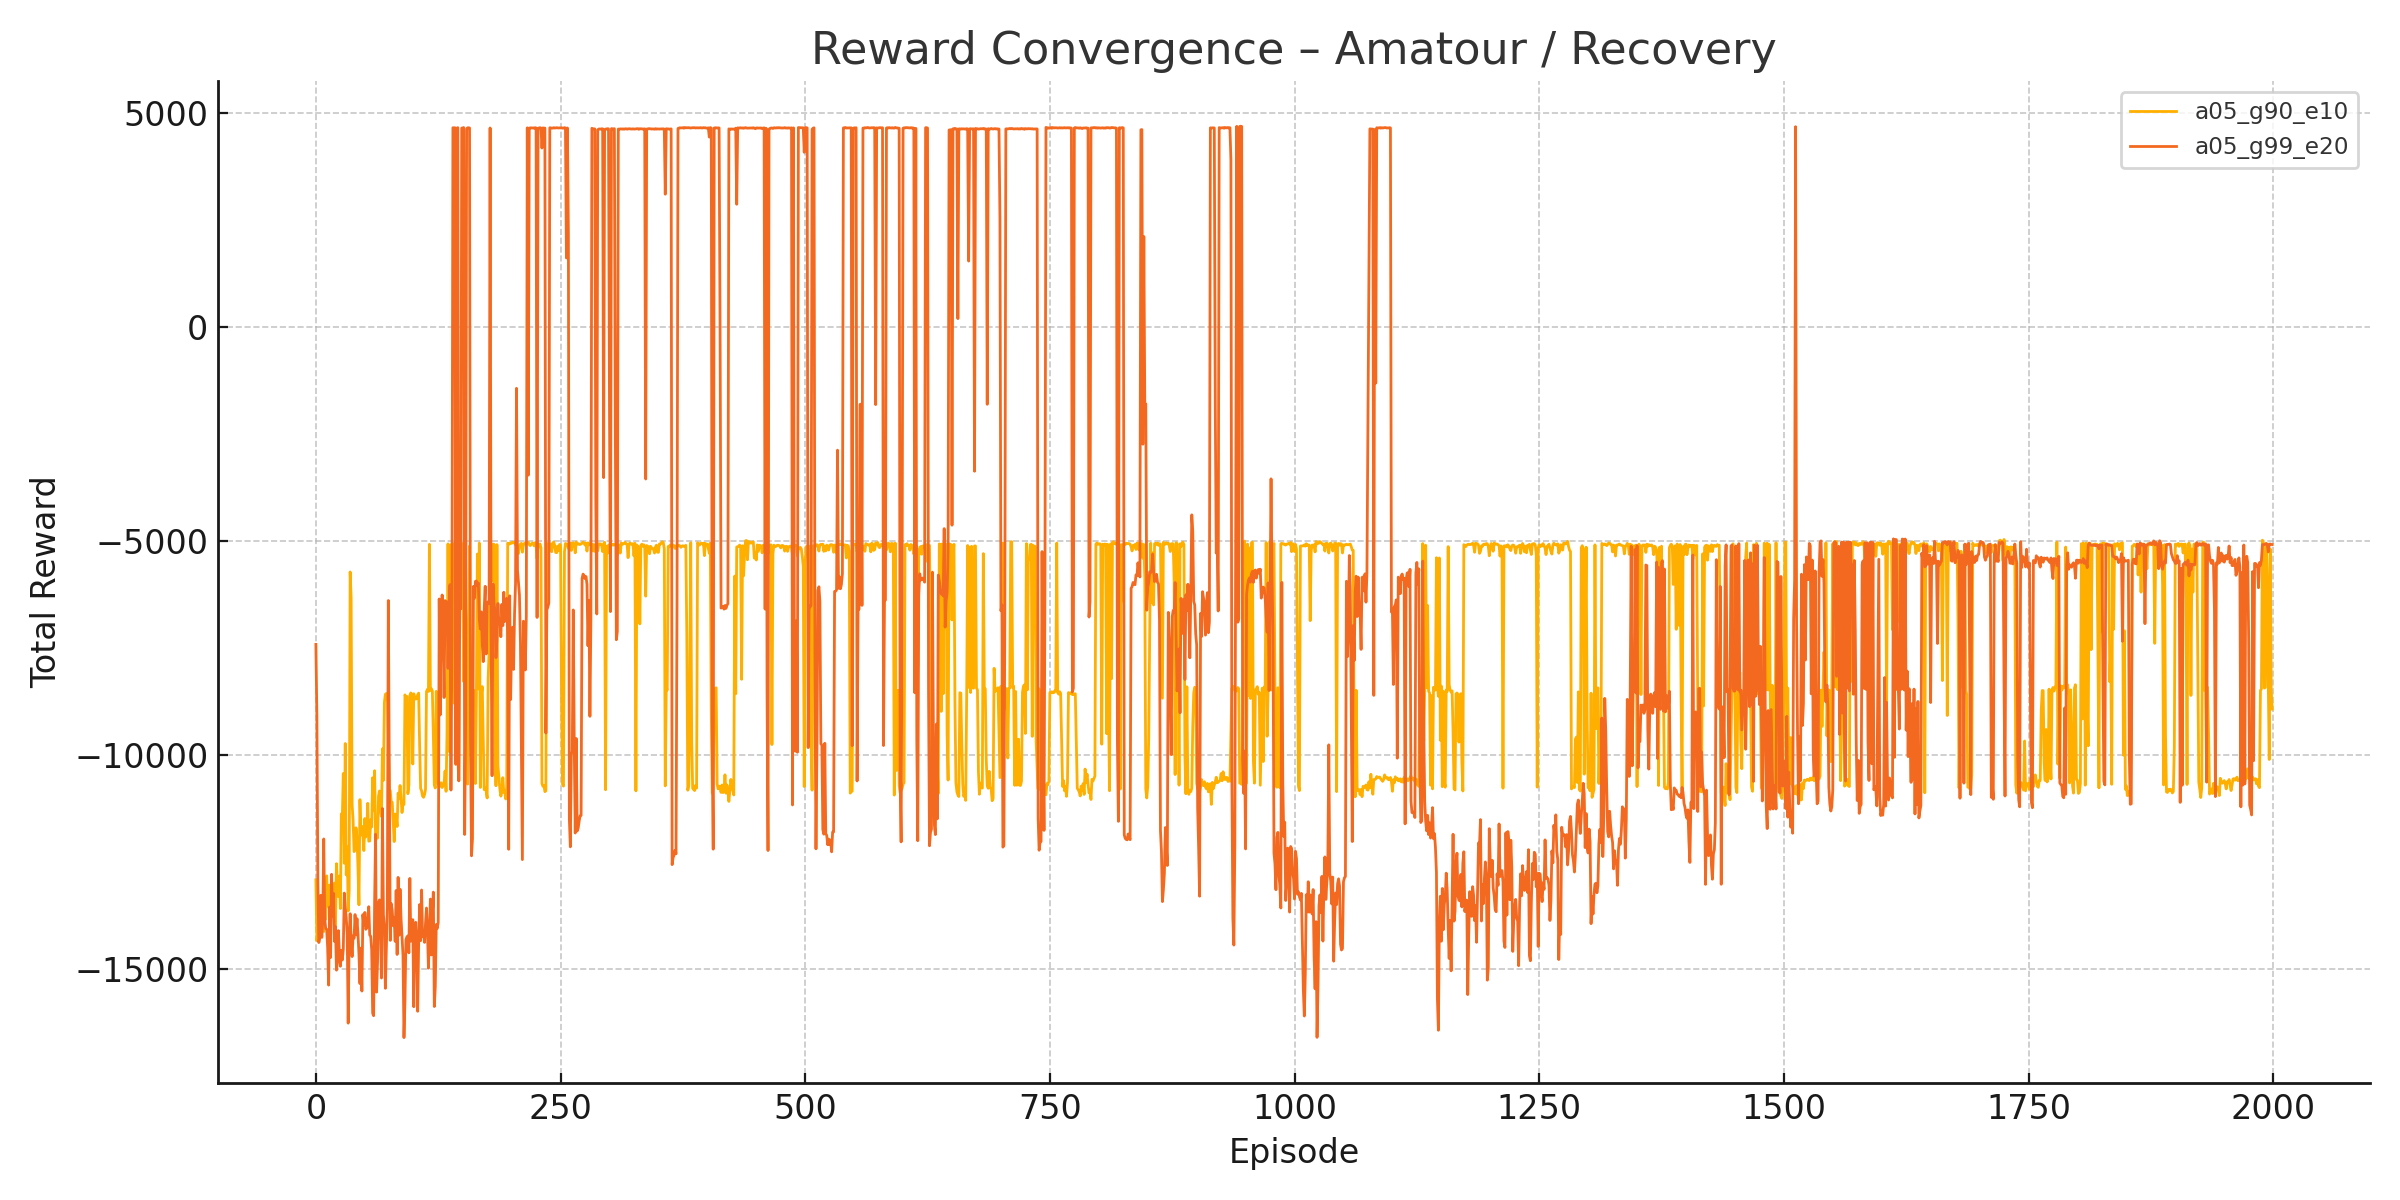
\includegraphics[width=\textwidth]{images/amatour_recovery_convergence.png}
    \caption{Recovery}
  \end{subfigure}
  \caption{Reward convergence for \textbf{amateur} (2000 episodes)}
  \label{fig:amateur_convergence}
\end{figure}


\subsection{Final Decision and Q-table Selection}

The second experiment identified the best hyperparameters for each athlete profile:

\begin{itemize}
    \item \textbf{Elite}:   \texttt{alpha=0.1, gamma=0.97, epsilon=0.5, decay=0.98}
    \item \textbf{Runner}:  \texttt{alpha=0.1, gamma=0.95, epsilon=0.2, decay=0.99}
    \item \textbf{amateur}: \texttt{alpha=0.05, gamma=0.90, epsilon=0.1, decay=0.98}
\end{itemize}
